\chapter{Upper Bound}
\label{ch:rel-ent}
\epigraph{To Infinity And Beyond}{Buzz Lightyear}

%\textcolor{red}{denk nochmal \"uber die struktur hier nach, also mit den
%numerischen approaches. naive approach zu den anderen? Auch auf simulations
%chapter verweisen!}
%
In this chapter we explore the approach of
\citeauthor{garrattProbingPostmeasurementEntanglement2023} presented in
\cite{garrattProbingPostmeasurementEntanglement2023}\footnote{While this
  reference points to a preprint on arXiv, we remark that the cited work has
since been published in
\citefield{garrattProbingPostmeasurementEntanglement2024}{journaltitle} with no
significant alterations (cf. ref.
\cite{garrattProbingPostmeasurementEntanglement2024})}. They introduce a method
to probe the critical point of the phase transition of a hybrid circuit. In
particular, they make use of Klein's inequality, bounding the entanglement
entropy from above. In the present chapter we introduce the idea behind this
approach, translate it to our system -- the projective transverse-field Ising
model (PTIM) --, and evaluate the quality of the resulting estimate. The
chapter is structured as follows. In \cref{sec:upperbound-idea} we state the
principles behind the idea and derive the upper bound. Moreover, we state and
prove that for Clifford circuits, i.e. in the stabilizer formalism, there is
only a limited class of cases, where the upper bound is non-trivial. In
\cref{sec:upperbound-numerics} we introduce different numerical post-processing
algorithms, trying to combat infinities appearing, when introducing an error
model akin to the one in \cref{sec:errormodel}. The results of which are shown
and discussed in \cref{sec:upperbound-results}. Finally, we provide and discuss
regularizations of divergences, weighing out utility and computational
efficiency.

%computable quantities
%In this chapter we investigate if Klein's Inequality can assist us in obtaining
%a sensible upper bound for the entanglement entropy and thus make the
%entanglement transition visible.
%
%Idea from Altman Paper:
%\citetitle{garrattProbingPostmeasurementEntanglement2023}
%\cite{garrattProbingPostmeasurementEntanglement2023}.
%In \cite{garrattProbingPostmeasurementEntanglement2023} they introduce a method
%to obtain an upper bound on the entanglement entropy via classical
%post-processing.
%
\clearpage
\section{The Idea \& Stabilizers}\label{sec:upperbound-idea}
In this section we will introduce the upper bound on entanglement entropy,
provide an information-theoretic interpretation and derive an expression for
the quantity of interest in case of stabilizer states. First however, we will
recall the definitions of some important quantities.
\subsubsection{Entropy of entanglement}
The main quantity of interest in the whole field of entanglement transitions is
the entropy of entanglement. It is a measure for how entangled one subsystem of a
bipartite state $\ket{\phi}_{AB}$ is with the other. We recall from
\cref{sec:ent-trans} that its definition can be stated as follows
\cite{fattalEntanglementStabilizerFormalism2004}.
\begin{defn}[Entanglement entropy]\label{defn:entanglement-entropy}
  Let $\ket{\phi}\in H^{\otimes N}$ be a bipartite pure state with subsystems
  $A$ and $B$. The entropy of entanglement of $\ket{\phi}$ then reads
  \begin{align}
    %&S_E : H^{\otimes N} \to [0, N/2]\nonumber\\
    S_\mathrm{E}\left(\ket{\phi}\right) \equiv - \Tr[\rho_B \log \rho_B],
  \end{align}
  where $\rho_B = \Tr_A[\dyad{\phi}]$ is the reduced density matrix of subsystem
  $B$. Conventionally, one uses the logarithm of base 2.
\end{defn}
This quantity can be efficiently computed in clifford circuits via the
stabilizer formalism. It is important to note that the density matrix of the
whole system $\rho = \dyad{\phi}$ describes a pure state. For a more universal
measure of entropy, where the entropy of entanglement is a special case, we
need to consider the more general \emph{von Neumann entropy}.
\subsubsection{Von Neumann entropy}
The von Neumann entropy lets us quantify the average information content in a mixture of
quantum states. Originally, von Neumann introduced it as an extension of the
classical Shannon entropy to quantum systems, as density matrices serve as
extension of the classical notion of (discrete) probability distributions
\cite{vonneumannMathematischeGrundlagenQuantenmechanik1968}.\footnote{Shannon
  entropy is a measure of the average information of probabilistic events.
  Since Information is defined as $I=-\log p_x$ for some event $x$ with
  probability $p_x$, we can write down an average, $S = \expval{-\log p_x}_x =
  -\sum_x p_x \log p_x$, which defines the Shannon entropy
\cite{shannonMathematicalTheoryCommunication1948}.} 
Consequently, we can write down a definition of the von Neumann entropy.
\begin{defn}[Von Neumann entropy]\label{defn:vonneumann}
  Let $\rho$ be an $N$-qubit density matrix. The von Neumann entropy of $\rho$
  is given by
  \begin{align}\label{eq:entropy-vn}
    S\left(\rho\right) \equiv \expval{-\log \rho} = -\Tr[\rho\log\rho]
  .\end{align}
\end{defn}
For diagonalizable matrices (as we expect density matrices to be) we can also
express \cref{eq:entropy-vn} as a sum over eigenvalues $\lambda_k$ of $\rho$, i.e.
\begin{align}\label{eq:entropy-vn-sum}
  S\left(\rho\right) = -\sum_k \lambda_k \log \lambda_k
,\end{align}
where $0\leq\lambda_k\leq 1$.
This can be shown by diagonalizing $\rho$ and using the fact that the matrix
logarithm of a diagonal matrix is just the logarithm of the entries.
(Note that we set $0\cdot\log 0 \equiv 0$.)

From this definition we can already derive some important properties, namely
its lower and upper bound. Firstly, $S(\rho)$ is non-negative and $0$ iff.
$\rho$ is pure. It is easy to convince oneself of that fact; for pure states we
have $\rho = \dyad{\phi}$, which has only one non-zero eigenvalue, $\lambda =
1$. Consequently, \cref{eq:entropy-vn-sum} reduces to $S(\rho) = - 1\cdot\log 1
=0$.  Next, $S(\rho)$ is maximal for the maximally mixed state. In a
$d$-dimensional Hilbert space, the density matrix of the maximally mixed state
is $\rho = \mathds{1}/d$. Hence, \cref{eq:entropy-vn-sum} reduces to
\[
  -\sum_k \frac{1}{d} \log \frac{1}{d} = -\log \frac{1}{d} = \log d
.\]
%One property we want to emphasize in particular is that $S(\rho)$ is bounded
%from above and below; it is $0$ for a pure state and $\log d$ for a maximally
%mixed state in a $d$-dimensional Hilbert space.
\subsubsection{Quantum relative entropy}
Lastly, we want to introduce the quantum relative entropy. 
%In classical
%information theory the relative entropy of one probability distribution $p_x$
%to another distribution $q_x$ provides a measure of excess information.
%Lost in the sense that if one assumes $q_x$ as the probability distribution
%over some sample space, where 
The same way we
motivated the von Neumann entropy, we want to define a quantum mechanical
analogue to the classical relative entropy. This quantity will play a role of
major importance in this chapter and is defined as follows.

\begin{defn}[Quantum relative and cross entropy]\label{defn:rel-ent}
  Let $\rho$ and $\sigma$ be density matrices with identical dimension. The
  relative entropy of $\rho$ to $\sigma$ is
  %$S: H^{\otimes N} \times H^{\otimes N} \to \mathbb{R}^+_0 \cup \{\infty\}$
  \begin{align}\label{eq:rel-ent-defn}
    S\left(\rho\mid\mid\sigma\right) \equiv \Tr[\rho\log\rho] -
    \Tr[\rho\log\sigma] = -S(\rho) - \Tr[\rho\log\sigma]
  ,\end{align}
  with the von Neumann entropy $S(\rho)$.
  The last term in \cref{eq:rel-ent-defn}, that is, 
  \begin{align}
    S\left( \rho\mid\mid\sigma \right) + S(\rho) \equiv S_C(\rho\mid\mid\sigma) = -\Tr[\rho\log\sigma]
  .\end{align}
  is known as \emph{cross entropy}. 
\end{defn}

Relative entropy, classical or quantum, quantifies excess surprisal when
one assumes $\sigma$ as a state\footnote{or probability distribution in the
classical case}, when the actual state is $\rho$. In that sense it tells us how
different two quantum states are. Interpreting it in this way also provides us
with a neat heuristic approach to possible values: the only way we do not lose
information is if we assume correctly, and in any other case we lose some. The
most extreme form of this is if $\mathrm{supp}(\rho)\cap\mathrm{ker}(\sigma)={0}$, where the
relative entropy diverges. In most general terms the relative entropy fulfils
\begin{align}\label{eq:inf-cond}
  S(\rho\mid\mid\sigma) < \infty \Longleftrightarrow \mathrm{supp}(\rho) \subseteq
  \mathrm{supp}(\sigma)
,\end{align}
where supp$(\bullet)\equiv\ $ker$(\bullet)^\perp$ is the support of a linear
operator, which is defined as the orthogonal complement to the kernel.
Alternatively, for diagonalizable matrices, it is the subspace spanned by
eigenvectors with non-zero eigenvalues
\cite{leditzkyRelativeEntropiesTheir2016,schumacherRelativeEntropyQuantum2000}.
This condition can be interpreted in a physical way. Let
\[
  \rho = \sum_i \lambda_i \dyad{\lambda_i} \quad{\text{and}} \quad
  \sigma = \sum_i \mu_i \dyad{\mu_i}
\]
be orthonormal eigendecompositions of $\rho$ and $\sigma$.
Then $S(\rho\mid\mid\sigma)$ diverges iff. there are states that $\rho$
features in its mixture that $\sigma$ doesn't. That is, $\rho$ has to be more
mixed than, or at least as mixed as, $\sigma$. If it is as mixed as
$\sigma$, it has to be a mixture of the same states. This means that the
information lost under the assumption of a purer state is infinite.
Since we know the von Neumann entropy to be bounded, this divergence occurs
solely in the $-\Tr[\rho\log\sigma]$ term. 

One property hinted at earlier is the non-negativity of the relative entropy.
This property goes by many different names, depending on context. For instance,
in classical statistical mechanics, this result is known as the \emph{Gibbs
inequality}. Its quantum mechanical analog is also known as \emph{Klein's
inequality}.
\subsection{Klein's inequality}
In this section we will state and prove the relation central to this chapter.
Its statement reads as follows.
\begin{thm}[Klein's inequality]\label{thm:kleins-ineq}
  The quantum relative entropy is non-negative, $S(\rho\mid\mid\sigma)\geq 0$, with equality iff.
  $\rho=\sigma$.
\end{thm}
While the statement in itself is written out rather simply, proving
\cref{thm:kleins-ineq} requires
us to introduce two auxilliary relations, namely \emph{Jensen's inequality} and
the \emph{log sum inequality}.
%Before we can go about proving \cref{thm:kleins-ineq}, we first need to
%introduce two auxilliary statements, which will be proven in the following.
%non-negativity of the classical relative entropy first. To this end, we introduce and
%prove some auxilliary lemmata, beginning with Jensen's inequality.
\begin{thm}[Jensen's inequality]\label{thm:jensen}
  Let $f$ be a convex function, that is, $f\left(\lambda x_1 + \left(
  1-\lambda \right)x_2\right) \leq \lambda f\left( x_1 \right) + \left(
  1-\lambda \right) f(x_2)$ with $0\leq\lambda\leq1$, and $X$ a discrete random
  variable. Then
  \begin{align}
    \mathbb{E}\left[f(X)\right] \geq f\left( \mathbb{E}\left[X\right] \right)
  .\end{align}
\end{thm}
\begin{proof}[Proof of Jensen's inequality]
  We will prove Jensen's inequality by induction over the mass of $X$.
  Associated with each event $x_i \in X$ is its probability $p_i$, such that
  our induction hypothesis is
  \begin{align}\label{eq:ind-hyp}
    \sum_{i=1}^n p_i f\left(x_i\right) \geq f\left(\sum_{i=1}^n p_i x_i
    \right).
  \end{align}
  As base case we have $n=2$;
  \begin{alignat*}{2}
    \mathbb{E}\left[f(X)\right] 
      &= p_1 f(x_1) + p_2 f(x_2) \\
      &= p_1 f(x_1) + (1-p_1) f(x_2) &&\qquad{\text{(Kolmogorov)}}\\
      &\geq f(p_1x_1 + (1-p_1)x_2) &&\qquad{(f\text{ convex})}\\
      &= f(\mathbb{E}[X])
  .\end{alignat*}
  For the induction step, assume \cref{eq:ind-hyp} holds for some
  $n\in\mathbb{N}_{>1}$, it must then also hold for $n+1$;
  \begin{alignat*}{2}
    \sum_{i=1}^{n+1} p_i f(x_i) 
      &= p_{n+1} f(x_{n+1}) + \sum_{i=1}^n p_i f(x_i)\\
      &= p_{n+1} f(x_{n+1}) + (1-p_{n+1})\sum_{i=1}^n \frac{p_i}{1-p_{n+1}} f(x_i)\\
      &\geq p_{n+1} f(x_{n+1}) + (1-p_{n+1})f\left(\sum_{i=1}^n
  \frac{p_i}{1-p_{n+1}} x_i\right) &&\qquad{\text{(Induction hypothesis)}}\\
      &\geq f\left(p_{n+1}x_{n+1} + (1-p_{n+1})\sum_{i=1}^n \frac{p_i}{1-p_{n+1}} x_i\right)
      &&\qquad{(f\text{ convex})}\\
      &=f\left(\sum_{i=1}^{n+1}p_i x_i\right).
  \end{alignat*}
  Since the base case and the induction step hold, we conclude that it holds
  $\forall n \in \mathbb{N}_{>1}$.
\end{proof}
\begin{cor}[Log sum inequality]\label{cor:logsum}
  Let $a_1, \ldots, a_n, b_1, \ldots, b_n \geq 0$ and let $a = \sum_i a_i$ and
  $b = \sum_i b_i$. Then
  \begin{align}\label{eq:logsum}
    \sum_{i=1}^n a_i \log \frac{a_i}{b_i} \geq a \log \frac{a}{b}
  .\end{align}
\end{cor}
\begin{proof}
  Let $f(x)=x\log x$. It is easy to convince oneself that $f$ is convex, and
  that it lets us rewrite the left side of \cref{eq:logsum}. We then have
  \begin{alignat*}{2}
    \sum_i a_i \log \frac{a_i}{b_i}
      &=\sum_i b_i f\left( \frac{a_i}{b_i} \right) 
      =b\sum_i \frac{b_i}{b} f\left( \frac{a_i}{b_i} \right) \\
      &\geq b\cdot f\left( \sum_i \frac{b_i}{b}\frac{a_i}{b_i} \right)
      &&\qquad{\text{(\cref{thm:jensen})}}\\
      &= b\cdot f\left( \frac{1}{b}\sum_i a_i \right)
      = b\cdot f\left( \frac{a}{b}\right) \\
      &= a \log \frac{a}{b}
  .\end{alignat*}
%  We can apply Jensen's inequality, since $\sum_i \frac{b_i}{b} = 1$ can be
%  taken as an average.   
\end{proof}
%Before we state the proof of \cref{thm:kleins-ineq} 
We now have all the tools ready to prove \cref{thm:kleins-ineq}. Our proof
follows the one laid out in \cite{nielsenQuantumComputationQuantum2010}, with
slight modifications.
\begin{proof}[Proof of \cref{thm:kleins-ineq}]
  Let $\rho=\sum_i p_i \dyad{i}$ and $\sigma=\sum_j q_j \dyad{j}$ be
  orthonormal decompositions for $\rho$ and $\sigma$. From \cref{defn:rel-ent}
  we can write
  \begin{align}\label{eq:ke-proof1}
    S(\rho\mid\mid\sigma) = \sum_i p_i \log p_i - \sum_i \bra{i} \rho
    \log\sigma \ket{i}
  .\end{align}
  With the eigendecomposition of $\rho$ and $\sigma$ we can write $\bra{i} \rho = p_i
  \bra{i}$ and
  \begin{align}\label{eq:ke-proof2}
    \expval{\log\sigma}{i} = \expval{\left(\sum_j \log q_j \dyad{j}
    \right)}{i} = \sum_j P_{ij}\log q_j  
  ,\end{align}
  with $P_{ij} = \ip{i}{j}\ip{j}{i} \geq 0$. 
  Plugging this into \cref{eq:ke-proof1} yields
  \begin{align}\label{eq:ke-proof3}
    S(\rho\mid\mid\sigma) = \sum_i p_i \left(\log p_i - \sum_j P_{ij} \log q_j \right)
  .\end{align}
  Note that $P_{ij}$ satisfies $\sum_i P_{ij} = \sum_j P_{ij} = 1$. We can thus
  interpret the last term in \cref{eq:ke-proof3} as an average of $-\log q_j$.
  Since $-\log$ is a strictly convex function it follows from \cref{thm:jensen}
  that
  \begin{align}
    -\sum_j P_{ij} \log q_j \geq - \log r_i
  ,\end{align}
  where $r_i = \sum_j P_{ij} q_j$, with equality iff. there exists a value of
  $j$ where $P_{ij}=1$. This implies 
  \begin{align}
    S(\rho\mid\mid\sigma) \geq \sum_i p_i \log\frac{p_i}{r_i}
  ,\end{align}
  where the equality occurs iff. there exists a $j$ with $P_{ij}=1$, i.e. iff.
  $P_{ij}$ is a permutation matrix.

  By \cref{cor:logsum} and the double stochasticity of $P_{ij}$ we obtain the
  final result
  \begin{align}
     S(\rho\mid\mid\sigma) \geq \sum_i p_i \log\frac{p_i}{r_i} \geq 1\cdot \log
     \frac{1}{1} = 0
  .\end{align}
\end{proof}

This result is essentially already our upper bound on the entanglement entropy,
since we have
\begin{align}
  \label{eq:kleins-ineq}
  S(\rho \mid\mid \sigma) \geq 0 \Leftrightarrow -\Tr[\rho\log\sigma]\geq
  S\left( \rho \right) 
\end{align}
with the relative and von Neumann entropy $S(\rho\mid\mid\sigma)$ and
$S(\rho)$ respectively. Since the von Neumann entropy is a more general form of
the entanglement entropy, we can employ Klein's inequality to upper bound the
entanglement entropy as well and thus try to find a signature of the phase
transition.

This idea was used in \cite{garrattProbingPostmeasurementEntanglement2023} for
a hybrid circuit of Haar random 2-qubit unitaries and $Z$ measurements. Since
they investigate a hybrid circuit, they take additional steps to circumvent the
post-selection problem, such as shadow tomography. To test their approach they
simulate their circuits with matrix product state (MPS) simulations. These
allow for a broader spectrum of mixed states than stabilizers do, and it is
computationally expensive, but feasible, to diagonalize the density matrix and
take its logarithm, to then compute the cross entropy upper bound. In our case,
however, we investigate a random circuit consisting of pauli measurements only
and thus employ stabilizer simulations to run numerical experiments on a
classical computer. As already elaborated on in \cref{sec:stab-basics},
the stabilizer formalism allows for lots of elegant computational shortcuts,
allowing efficient quantum simulations on classical computers. Consequently,
one might ask if there also is an efficient way to compute the cross or
relative entropy. We will explore this question in the next section.

%Among other things, they make use of shadow tomography to circumvent the
%post-selection problem. 
%However, they do MPS simulations, and not stabilizer. This, of course, calls
%for an adaptation (oh well\ldots).
%\begin{itemize}
%  \item \cite{garrattProbingPostmeasurementEntanglement2024} do mps
%    simulations, which, as it turns out, have a broader spectrum of mixed states than stabilizer
%    states. 
%  \item thats why they need shadow tomography and stuff
%  \item also, they do a hybrid circuit with random haar unitaries
%  \item only one type of measurement and the probability refers to if any
%    measurement is performed (on the computational basis)
%  \item MPS has lower dimensions, it is computationally expensive, but
%    feasible, to diagonalize the density matrix and take its log
%  \item[$\to$] what about clifford circuits? is there a way to write out the
%    relative entropy for stabilizers? In fact, there is:
%\end{itemize}


\subsection{Stabilizers}\label{sec:rel-ent-stab}
When resarching the quantum relative entropy and cross entropy and possible
expressions thereof in the stabilizer formalism, we have not been successful in
finding an efficient method, such as the one for the entanglement entropy
(cf. ref. \cite{fattalEntanglementStabilizerFormalism2004})
\cite{veitchResourceTheoryStabilizer2014,niekampEntropicUncertaintyRelations2012,leoneStabilizerEntropiesAre2024,leonePhaseTransitionStabilizer2024,wuEntanglementUpperBound2011,vedralEntanglementMeasuresPurification1998,lindenQuantumEntropyCone2013,buExtremalityStabilizerStates2024,arabLectureNotesQuantum2024,nielsenQuantumComputationQuantum2010}.
In this section we will therefore examine the upper bound on the entanglement entropy
given by \cref{thm:kleins-ineq} in the context of stabilizers and the
stabilizer formalism. In particular, we will explore the condition of infinite
relative entropy,
provide and prove a necessary and sufficient condition
for $S(\rho\mid\mid\sigma)<\infty$ when $\rho$ and $\sigma$ are stabilizer
density matrices (\cref{prop:subgroup}), and derive an expression for finite cross
and relative entropy.

Recall that we have $S(\rho\mid\mid\sigma)<\infty$ for
supp$(\rho)\subseteq$ supp$(\sigma)$. For the proof of \cref{prop:subgroup} it
will prove useful to introduce an auxilliary lemma, which relates the support
of a density matrix to the stabilized subspace.
\begin{lem}\label{lem:supp-is-vs}
  Let $\rho$ be an $N$-qubit stabilizer density matrix with stabilizer group
  $\mathcal{S} = \langle
  g_1, \ldots, g_n \rangle$, and $0\leq n \leq N$.
  Then \[ \mathrm{supp}(\rho) = V_{S}.\]
\end{lem}
\begin{proof}[Proof of \cref{lem:supp-is-vs}]
  By definition (cf. \cref{ch:basics}) we take $V_{S}$ to be the vector space
  stabilized by $\mathcal{S}$.  Further, it is the intersection of subspaces fixed by
  each operator in $\mathcal{S}$, i.e. the eigenvalue one eigenspaces of
  elements of $\mathcal{S}$
  (cf. \cref{sec:stab-basics}). More
  formally we can write
  \[ 
    V_S = \bigcap_{g \in \mathcal{S}}  \left\{\ket{\psi} \mid g\ket{\psi} =
    \ket{\psi}\right\} = \left\{\ket{\psi} \mid g\ket{\psi} =
  \ket{\psi} \forall g \in \mathcal{S}\right\}.
  \]
  This subspace is projected onto by
  \[ \mathbb{P}_S \equiv \frac{1}{2^n} \prod_{g\in \mathcal{S}} \left(\mathds{1} + g\right).\]
  Recall from \cref{sec:stab-basics,defn:stab-dmat} that $\rho$ can be written as a product of
  projectors
  \[ \rho = \frac{1}{2^N} \prod_{g \in \mathcal{S}} \left(\mathds{1} + g\right)
  = 2^{n-N} \mathbb{P}_S \]
  We thus have
  \[ \mathrm{supp}(\rho) = \mathrm{supp}(\mathbb{P}_S) = V_S. \]
\end{proof}

\begin{thm}\label{prop:subgroup}
  Let $\rho$ and $\sigma$ be $N$-qubit stabilizer density matrices with
  respective stabilizer groups $\mathcal{S}_\rho$ and $\mathcal{S}_\sigma$. Then
  \[ \mathrm{supp}(\rho)\subseteq \mathrm{supp}(\sigma) \Longleftrightarrow
  \mathcal{S}_\sigma \leq \mathcal{S}_\rho. \]
  That is, with \cref{eq:inf-cond}, $S(\rho\mid\mid\sigma)$ takes on finite
  values iff. $\mathcal{S}_\sigma$ is a
  subgroup of $\mathcal{S}_\rho$.
\end{thm}

\begin{proof}[Proof of \cref{prop:subgroup}]
  We will prove implication from both directions to prove equivalence.

  \enquote{$\Leftarrow$} Let $\mathcal{S}_\sigma \leq \mathcal{S}_\rho$. Then
  \begin{align*}
    \mathrm{supp}(\rho) = V_{S,\rho} &= \bigcap_{g\in S_\rho} \left\{ \ket{\psi} \mid
    g\ket{\psi} = \ket{\psi} \right\} \\
        &\overset{S_\sigma \leq S_\rho}{=} \underbrace{\bigcap_{g\in S_\sigma}
        \left\{\ket{\psi} \mid g \ket{\psi} =
        \ket{\psi}\right\}}_{V_{S,\sigma}}\ \ \ \cap \bigcap_{g \in S_\rho \setminus
        S_\sigma} \left\{\ket{\psi} \mid g \ket{\psi} =
        \ket{\psi}\right\}\\
        &= V_{S,\sigma} \cap \bigcap_{g \in S_\rho \setminus
        S_\sigma} \left\{\ket{\psi} \mid g \ket{\psi} =
        \ket{\psi}\right\}\\
        &\subseteq V_{S,\sigma} = \mathrm{supp}(\sigma)
  .\end{align*}
  which finishes the proof of this direction.

  \enquote{$\Rightarrow$} Let $V_{S,\rho} = \mathrm{supp}(\rho) \subseteq
  \mathrm{supp}(\sigma) = V_{S,\sigma}$. 
  For the proof of this direction, consider the relations between the subspaces
  of the $N$-qubit Hilbert space $H^{\otimes N}$ outlined in the following
  diagram.
  \begin{figure}[H]
    \centering
  \begin{tikzpicture}
  \matrix (m) [matrix of math nodes,row sep=3em,column sep=4em,minimum width=2em]
  {
    H^{\otimes N} & V_\rho \\
     V_\sigma &  \\};
  \path[-stealth]
    (m-1-1) edge node [left] {$\mathbb{P}_\sigma$} (m-2-1)
    edge node [above] {$\mathbb{P}_\rho$} (m-1-2)
    (m-2-1) edge node [below] {$\mathbb{P}_\rho$} (m-1-2);
  \end{tikzpicture}
\end{figure}

  We can read the diagram as follows: From the $N$-qubit Hilbert space we can
  project onto the vector space stabilized by $\mathcal{S}_\sigma$, $V_\sigma$, by means of a
  projection operator. Likewise we can do the same for $V_\rho$. Since we
  require $V_{S,\rho} \subseteq V_{S,\sigma}$, the same projection that takes
  us from $H^{\otimes N}$ to $V_{S,\rho}$ will take us from $V_{S,\sigma}$ to
  $V_{S,\rho}$. It follows that $\mathbb{P}_\sigma \mathbb{P}_\rho = \mathbb{P}_\rho$.

  Let $\ket{\psi} \in V_\rho$. We thus have
  \[
    \ket{\psi} = \mathbb{P}_\rho \ket{\psi} = \mathbb{P}_\sigma \mathbb{P}_\rho
    \ket{\psi} = \mathbb{P}_\sigma
    \ket{\psi}.
  \]
  Since $\ket{\psi}$ was an arbirtary element from $V_{S,\rho}$ and $\mathbb{P}_\sigma =
  \frac{1}{2^n} \prod_{i=1}^n \left(\mathds{1} + h_i\right)$ with $h_i \in
  \mathcal{S}_\sigma$ it follows that all stabilizers of $\sigma$ also stabilize $\rho$
  and thus
  \[
    \mathcal{S}_\sigma \leq \mathcal{S}_\rho.
  \]
%  $\ket{\psi} \in V_{S,\rho}$ and $\ket{\phi} \in
%  V_{S,\sigma} \setminus
%  V_{S,\rho}$. \"o Since the stabilizer group is the
%  symmetry group of $V_S$, we can rewrite $S_\sigma$ as
%  \[ 
%    S_\sigma = \left\{ g \in G_N \mid g \ket{\psi} = \ket{\psi} \wedge g\ket{\phi} =
%  \ket{\phi} \right\},
%  \]
%  (where $G_N$ is the $N$-qubit Pauli group) 
%  as we want $S_\sigma$ to stabilize both $V_{S,\sigma}$ and its subset
%  $V_{S,\rho}$. We can then split up the condition into the intersection of two
%  sets, i.e.
%  \begin{align*}
%    S_\sigma &= \left\{ g \in G_N \mid g \ket{\psi} = \ket{\psi} \wedge g\ket{\phi} =
%  \ket{\phi} \right\}\\
%             &= \underbrace{\left\{ g \in G_N \mid g\ket{\psi}= \ket{\psi}
%             \right\}}_{S_\rho} \cap \left\{ g \in G_N \mid g\ket{\phi} = \ket{\phi} \right\} \\
%             &= S_\rho \cap \left\{ g \in G_N \mid g\ket{\phi} = \ket{\phi} \right\} \\
%               &\leq S_\rho 
%  .\end{align*}
  This concludes the proof.
\end{proof}
We have thus shown that that the condition for finite values of the relative
entropy is equivalent to a simple statement about the group structure of the
respective stabilizer groups. Furthermore, we know from 
\cite{fattalEntanglementStabilizerFormalism2004} that the entropy of
entanglement can be expressed in a simple way through group properties.
We'd like for this to also be the case for other entropic quantities,
especially the cross and relative entropy, which are our main concern.

It turns out that one can indeed derive expressions for the cross and relative
entropy that put these information-theoretic quantities in a relation with
abstract group properties. Confer with
\cref{thm:cross-ent-stab,col:rel-ent-stab} for the precise statements. The
resulting expressions are remarkable in their simplicity, as well as their
similarity to each other and to previous results. As a warm-up for the proofs
of \cref{thm:cross-ent-stab,col:rel-ent-stab} we will derive an expression for
the von Neumann entropy in the stabilizer formalism first. This will also aid
in the derivation of the expression for relative entropy, since it is a
difference of the cross and von Neumann entropy.

\begin{lem}[Von Neumann entropy -- stabilizers]\label{lem:vn-ent-stab}
  Let $\rho$ be an $N$-qubit stabilizer density matrix with stabilizer group
  $\mathcal{S}_\rho$ and rank $\abs{\mathcal{S}_\rho} \equiv r$. Then
  \begin{align}
    S\left( \rho \right) = N - r
  .\end{align}
\end{lem}
\begin{proof}
  Let $\mathcal{S}_\rho$ be an $N$-qubit stabilizer group of rank $r$ with
  corresponding density matrix $\rho$.

  By \cref{defn:vonneumann}, or \cref{eq:entropy-vn-sum} in particular, we have
  \begin{align}\label{eq:entropy-vn-sum-proof}
    S\left( \rho \right) = -\Tr[\rho\log\rho] = -\sum_k \lambda_k \log
    \lambda_k
  .\end{align}
  Thus, we need to diagonalize, i.e. find the eigenvalues $\lambda_k$ of
  $\rho$.

  Since $\rho$ is a stabilizer density matrix, it can -- up to a constant
  multiple -- also be written as a
  product of projectors onto the $+1$ eigenspaces of group generators
  \begin{align}
    \rho = \frac{1}{2^N} \prod_{i=1}^r (\mathds{1} + g_i) = 2^{r-N} \mathbb{P}_\rho
  .\end{align}
  Knowing that projections are diagonalizable with eigenvalues of either $0$ or
  $1$, we know that the diagonal form of $\rho$ is the diagonal form of
  $\mathbb{P}_\rho$ with a constant multiple $2^{r-N}$, that is\footnote{Note that
    the bottom right entry need not be zero. This specific choice was made for
  illustratory purposes.}
  \begin{align}
    D_\rho = 2^{r-N} \mqty(\dmat{1,\ddots,0})
  .\end{align}
  With $\Tr[\rho] = 1$ it follows that the eigenvalues of $\rho$ must be
  $\lambda_k = 2^{r-N}$ for $k =1,\ldots,2^{N-r}$ and
  $\lambda_k = 0$ for all other $k$.
  Inserting this back into \cref{eq:entropy-vn-sum-proof} yields
  \begin{align*}
    S\left( \rho \right) 
      &= -\sum_{k=1}^{2^N} \lambda_k \log \lambda_k 
      = -\sum_{k=1}^{2^{N-r}} 2^{r-N} \log 2^{r-N} 
      = -2^{N-r} 2^{r-N} \log 2^{r-N} 
      = -\log 2^{r-N} \\
      &= N-r
  .\end{align*}
\end{proof}
The expression of the von Neumann entropy is not only interesting going
forward, e.g. in the derivation of the relative entropy, but also from a group
theoretic perspective. That is, it should be noted that by asking an
information-theoretic question, we got a group theoretic answer. Let us
convince ourselves that it is a reasonable one, by testing it on our intuition
on entropy.

With $N$ qubits we have a generating set of size $N$, at most. In the case
where we have $N$ generators, the state associated with the stabilizer group is
a pure state, and the entropy should be $0$, which is the case for $r=N$. For
the maximally mixed state, the generating set is the empty set and the
stabilizer group the trivial group. In accordance to our expectations, this
should yield $\log(2^N)= N$ for the von Neumann entropy. Indeed, since the size of
the empty set is $0$, we have that $r=0$ and thus $S(\rho) = N$.

Removing one generator thus increases entropy by $1$, or put differently,
starting from the empty set and adding generators to it decreases entropy by
$1$ for each generator added. This too should come to no surprise, as we know
that for each generator removed (added) from a full set of stabilizers, we
double (halve) the stabilized state space, effectively creating (purifying) a
perfect mixture of stabilized states.

\begin{thm}[Cross entropy -- stabilizers]\label{thm:cross-ent-stab}
  Let $\rho$ and $\sigma$ be $N$-qubit stabilizer density matrices with
  respective stabilizer groups $\mathcal{S}_\rho$ and $\mathcal{S}_\sigma$ that
  satisfy $\mathcal{S}_\sigma \leq
  \mathcal{S}_\rho$. Further, let $\abs{\mathcal{S}_\sigma} \equiv s$. Then
  \begin{align}\label{eq:cross-ent-stab}
    S_C(\rho\mid\mid\sigma) = N - s
  .\end{align}
\end{thm}

\begin{proof}
   Let $\mathcal{S}_\rho$ and $\mathcal{S}_\sigma$ be $N$-qubit stabilizer
   groups that satisfy $\mathcal{S}_\sigma \leq \mathcal{S}_\rho$. Their
   respective density matrices can be written as
   \begin{align}
     \rho = \frac{1}{2^N} \prod_{i=1}^r (\mathds{1} + g_i) \quad{\text{and}}
       \quad \sigma = \frac{1}{2^N} \prod_{i=1}^s (\mathds{1} + h_i)
   \end{align}
   with $r \equiv \abs{\mathcal{S}_\rho}$ and $s \equiv
   \abs{\mathcal{S}_\sigma}$. Since we require $\mathcal{S}_\sigma \leq
   \mathcal{S}_\rho$, we can construct a generating set $G_\sigma$ of
   $S_\sigma$, where each element of $G_\sigma$ commutes with the generating
   set of $G_\rho$. Note that the generating sets are not necessarily
   identical. However, since $\mathcal{S}_\sigma$ is by construction a subgroup
   of $\mathcal{S}_\rho$, which in turn is an abelian subgroup of
   $\mathcal{P}_N$, all elements of $\mathcal{S}_\sigma$ commute with all elements of
   $\mathcal{S}_\rho$. It follows that the density matrices themselves also
   commute, i.e.
   \begin{align}
      \left[\rho, \sigma\right] = 0
   .\end{align}
   It is a well-known fact from linear algebra and functional analysis that
   commuting operators share a common eigenbasis and can be diagonalized
   simultaneously. We therefore write $\rho = UD_\rho U^{-1}$ and $\sigma =
   UD_\sigma U^{-1}$ with transformation matrix $U$ and corresponding diagonal
   matrix $D_{\rho / \sigma}$. We also have that the logarithm of a diagonalizable
   matrix is \cite{hallElementaryIntroductionGroups2000}
   $$\log \sigma = U \log D_\sigma U^{-1}.$$ Consequently,
   \begin{align}
      S_C(\rho\mid\mid\sigma) = -\Tr[\rho \log\sigma] = -\Tr[U D_\rho U^{-1} U \log D_\sigma U^{-1}] =
      -\Tr[D_\rho \log D_\sigma] 
   .\end{align}
   With $D_\rho$ and $D_\sigma$ diagonal we can write the trace as
   \begin{align}\label{eq:the-sum}
      -\Tr[D_\rho \log D_\sigma] = -\sum_k \lambda_k \log \mu_k
   \end{align}
   with the eigenvalues $\lambda_k$ and $\mu_k$ of $\rho$ and $\sigma$,
   respectively.

   As we know from the previous proof, $\lambda_k = 2^{r-N}$ for
   $k=1,\ldots,2^{N-r}$ and $0$ otherwise, and analogously, $\mu_k = 2^{s-N}$
   for $k=1,\ldots,2^{N-s}$ and $0$ otherwise. Note that the subgroup condition
   implies that $r\geq s$ or more specifically $N-r \leq N-s$. This ensures that to every non-zero entry in
   $D_\rho$ there is a corresponding non-zero entry in $D_\sigma$. In other
   words, for all $k$, $\lambda_k \neq 0 \Rightarrow \mu_k \neq 0$. More
   importantly for us, however, is the contrapositive, $\mu_k = 0 \Rightarrow
   \lambda_k = 0$, which tells us that any divergence that might occur
   in the logarithm gets intercepted by a leading factor of $0$.

   Inserting this into the sum in \cref{eq:the-sum} we get
   \begin{align}
      -\sum_i 2^{r-N} \log 2^{s-N} =
      -2^{N-r}2^{r-N}\left(s-N\right)= N-s
   ,\end{align}
   which concludes the proof.
\end{proof}

Although \cref{thm:cross-ent-stab,eq:cross-ent-stab} are in dire need to be
discussed, we do not want to fail to mention that the relative entropy between
two stabilizer density matrices follows as a corollary.

\begin{cor}[Relative entropy -- stabilizers]\label{col:rel-ent-stab}
  Let $\rho$ and $\sigma$ be $N$-qubit stabilizer density matrices with
  respective stabilizer groups $\mathcal{S}_\rho$ and $\mathcal{S}_\sigma$,
  where $\abs{\mathcal{S}_\rho}
  \equiv r$ and $\abs{\mathcal{S}_\sigma} \equiv s$. If $\mathcal{S}_\sigma \leq
  \mathcal{S}_\rho$ then the relative entropy of $\rho$ to
  $\sigma$ is
  \begin{align}
    S\left(\rho\mid\mid\sigma\right) = r - s
  .\end{align}
\end{cor}

\begin{proof}
  Let $\rho$ and $\sigma$ be density matrices satisfying the stated
  requirements, $\mathcal{S}_\sigma \leq \mathcal{S}_\rho$ in particular. From \cref{defn:rel-ent},
  or more precisely \cref{eq:rel-ent-defn}, we have
  \begin{align}
    S\left( \rho\mid\mid\sigma \right) = -S\left( \rho \right)
    -\Tr[\rho\log\sigma]
  .\end{align}
  Inserting our results from \cref{lem:vn-ent-stab,thm:cross-ent-stab} yields
  \begin{align}
    -S\left( \rho \right) -\Tr[\rho\log\sigma] = -(N-r) + N - s = r - s
  .\end{align}
\end{proof}

%What are the information-theoretic implications of \cref{thm:cross-ent-stab}?
Notice that although it is defined as a quantity relating $\rho$ to $\sigma$,
there is no explicit dependence of $\rho$ in \cref{eq:cross-ent-stab}.
What \cref{thm:cross-ent-stab} seems to imply is that the cross entropy between two stabilizer
density matrices $\rho$ and $\sigma$ just amounts to the von Neumann entropy of
$\sigma$. However, this is where one needs to be careful. While the resulting
numerical value is entirely dependent on $\sigma$ and its stabilizer group
alone, we have an implicit dependence through the requirement that
$\mathcal{S}_\sigma \leq \mathcal{S}_\rho$. Since we were able to show that the
cross entropy is infinite in the converse case (cf. \cref{prop:subgroup}), we
could add the $\rho$ dependence back in, i.e.
\begin{align}
  -\Tr[\rho\log\sigma] = \begin{cases}
    N - \abs{\mathcal{S}_\sigma} &\quad{\mathcal{S}_\sigma \leq
    \mathcal{S}_\rho}\\
      \infty &\quad{\mathcal{S}_\sigma \not\leq \mathcal{S}_\rho}
  \end{cases}
.\end{align}
This detail will be important later on, as we try to avoid explicit
dependences on $\rho$, which would take us back to the sampling problem.

The independence of $\rho$ in the first case, however, is still quite a
remarkable result. Let's examine the expression and convince ourselves that
this simplicity is no accident.
From the subgroup condition we know that the state
described by $\sigma$ needs to be more mixed or at least as mixed as $\rho$.
That is, the probability distribution on the state space represented by $\sigma$ contains
more states than $\rho$. However, all states of $\rho$ are featured in
$\sigma$ with uniform probability. Any state in the mixture of $\sigma$ thus
gets assigned the same weight when averaging. Additionally, the probabilities
over the larger state space are uniformly distributed as well, turning $\log
\mu_k$ into a constant factor. It is therefore an average of a constant over a
uniform probability distribution, which is just the constant itself. 

%
%\textcolor{red}{Something something, cross entropy independent of $\rho$,
%  essentially the von neumann entropy of $\sigma$, which is, dare I say,
%rather trivial compared to what one expects from a logarithmic quantity}

We have discussed the mathematical and information-theoretic aspect of the
derived statements, but we should also think about the physical
implications of these statements. Although we summarized the idea, we want to
reemphasize the utility behind these expressions.
Our ultimate goal is an upper bound on the half-system
entanglement entropy, $S_E\left( \rho \right)$,\footnote{Here, $\rho$ refers to
the reduced density matrix of half the system, where the entire system is in
the pure state $\ket{\phi}$} which can be derived from \cref{eq:kleins-ineq}.
With that, we try to detect a signature of the critical point of the phase
transition found by classical simulations. Recall that the half-system
entanglement entropy is non-linear in the density matrix, that is, it is an
observable of the state itself, requiring exponentially many copies of the same
state. Therefore, it is infeasible, and practically impossible, to perform
measurements quantifying entanglement with the entanglement entropy. However,
by \cref{eq:kleins-ineq} we can obtain an upper bound, $S_E\leq
-\Tr[\rho\log\sigma]$, thus circumventing the sampling problem. The choice of
$\sigma$ has some degree of arbitraryness; as long as 
$\mathrm{supp}\left( \rho \right) \subseteq \mathrm{supp}\left( \sigma \right)$ 
we get a finite upper bound, and even have equality if $\rho = \sigma$.  But
this is not the whole picture. It stands to reason that we \emph{should} be
picky with our choice of $\sigma$ and be consistent with it.  In particular, we
ideally would like to relate $\sigma$ to the experimental state
$\rho$ in some way or another. This can be done by classically reconstructing
$\rho$ by means of projecting the measurement outcomes from the record
$\mathbf{m}$. Then, by tracing out half of the system, we obtain some
$\sigma$, which we can use in the upper bound. The classical post-processing of
the measurement record requires us to efficiently simulate the system, as well
as to be able to project onto specific outcomes. 
To this end, we prefer to use
stabilizer simulations, as they allow the efficient simulation and
post-processing of our system. With \cref{thm:cross-ent-stab} we now
additionally have an efficient method of computing the upper bound to the
entanglement entropy, such that the inequality becomes
\begin{align}
  S_E \leq N-s
.\end{align}
The following sections therefore pertain to the various possible
post-processing algorithms one might make use of. 
%\subsection{Shadow Tomography}
%these papers are cited in
%\cite{garrattProbingPostmeasurementEntanglement2023} for shadow tomography:
%\begin{itemize}
%  \item \citetitle{elbenRandomizedMeasurementToolbox2022}
%    \cite{elbenRandomizedMeasurementToolbox2022}
%
%    Review paper. Context: "It will be useful to first outline shadow
%    tomography \cite{elbenRandomizedMeasurementToolbox2022} in its simplest
%    incarnation for a single qubit"
%
%    It has indeed been useful, but I gotta admit, i didn't get my outline from
%    this one, but from:
%  \item \citetitle{huangPredictingManyProperties2020}
%    \cite{huangPredictingManyProperties2020} 
%
%    In this paper, shadow tomography is the main thing investigated. Context:
%    "Generalizing \ldots to multiple qubits is straightforward
%    \cite{huangPredictingManyProperties2020}: one possibility is to construct
%    $N$-qubit shadows as the tensor products of $N$ objects with the structure
%    \ldots"
%\end{itemize}
%
%Some more shadow tomography papers:
%\begin{itemize}
%  \item \cite{aaronsonShadowTomographyQuantum2018} shadow tomography defined
%    for the first time
%  \item IDK where i want to include this one, but i think it will be
%    interesting to study a bit more:
%    \cite{tothEntanglementDetectionStabilizer2005} Entanglement witness
%\end{itemize}
%
%This one is not on shadow tomography, but is cited in
%\cite{garrattProbingPostmeasurementEntanglement2023}, which got me hella
%frustrated, since I did not know what the hell they meant with "Our discussion
%in this section largely follows Ref.
%\cite{garrattMeasurementsConspireNonlocally2023}" if it does not really match
%the vibe of \emph{this section}.
%


\section{Naive approach}\label{sec:naive-approach}
The key idea of the upper bound is to have a quantity that is linear in $\rho$.
By obtaining a measurement record $\vb{m}$, we can try and classically
reconstruct the experimental density matrix $\rho$ from the record. Since we
are doing a classical computation, we have the advantage of being able to
project onto measurement results. We therefore can -- naively -- attempt a
reconstruction of our experiment based on the data. Of course, in our case, we
also use a classical simulator to generate data.

\subsection{Methods}
After the data has been generated we do as we did before in \cref{ch:lxe} and
project the measurement outcomes onto $\sigma$. However, we start from the same
state $\rho = \sigma = \dyad{GHZ+}$. After we have completed the circuit, we
trace out one half of the qubits and compute the cross entropy, which is given
by \cref{eq:cross-ent-stab}. 

For our prospective numerical experiments, we would therefore have them support
the simulation of mixed states, since we might encouter them by means of
partially tracing out the system. To this end, we refer to \cref{ch:mixed}, in
particular \cref{sec:mixed-states,sec:sim-entropies,sec:ptrace}. In these
sections, we introduce the algorithms used to realize mixed states, the
different entropic quantities, and the partial trace, respectively. Of course,
we additionally need to adapt the projection function, since we now
\emph{force} the projection upon the state. For the computation of the linear
cross entropy, it sufficed to know if projections were successful all the way
through. If they weren't, we would simply break the loop over the measurement
record and stop the projections. Here, we really want a faithful reconstruction
of the density matrix. The algorithm to force projections is outlined in
\cref{alg:force-project}.

As we use the general setup from \cref{ch:lxe}, we also employ the error model
introduced in \cref{sec:errormodel} to emulate noise in the circuit. This is to
ensure comparability between the general approaches of the linear cross entropy
and the cross entropy as upper bound.

As we have access to the \enquote{experimental} density matrix $\rho$ through
our numerical simulation, we employ the implementation of the cross entropy as
outlined in \cref{thm:cross-ent-stab}. An important detail to note however is
that we do not want infinities appearing in our data. As such, 
in the case of $\mathcal{S}_\sigma \not\leq
\mathcal{S}_\rho$, we add $N /2$, where $N$ is the number of qubits in the
system. This amounts to replacing the density matrix $\sigma$ by the maximally
mixed state.

\subsection{Results}

In \cref{fig:naive-svn-vs-se-no-error} the results of the upper bound is shown
in the case of no noise in the circuit.
\begin{figure}[t]
  \centering
  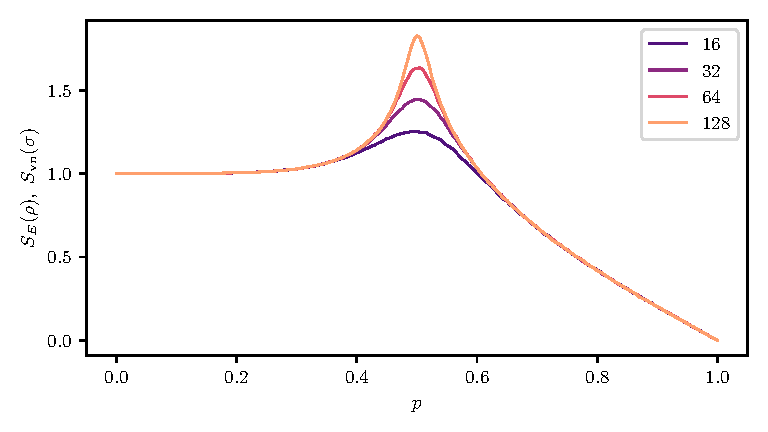
\includegraphics{naive_approach_cleansystem_soloplot.pdf}
  \caption{Cross and entanglement entropy in the noiseless system. We project
    the measurement outcomes from $\rho$ onto $\sigma$ if possible. Note that
    we here use periodic boundary conditions. Each datapoint corresponds to
    $\sim 10^5$ samples.}
  \label{fig:naive-svn-vs-se-no-error}
\end{figure}
\Cref{fig:naive-svn-vs-se-no-error} shows that there is perfect overlap between the original and
the replicated system in the noiseless case. This is also what one would
expect, since we effectively computed the entanglement entropy of a pure state that
happens to have had the same measurement record as $\rho$. And incidentally,
every outcome in the measurement record corresponded to an outcome that could
be projected perfectly onto $\sigma$. We thus perfectly saturated the upper
bound \cref{eq:kleins-ineq}. 

We now turn towards a more realistic scenario, namely that of a noisy circuit.
The error model we use to emulate noise is the one introduced in
\cref{sec:errormodel}. Note that we force the projections onto $\sigma$, and
thus should recover a close estimate of the experimental density matrix. If it
turns out that the density matrix obtained from the experiment does not have
support in $\sigma$, we replace the appearing infinity with $L /2$, where $L$
is the number of qubits.
\begin{figure}[t]
  \centering
  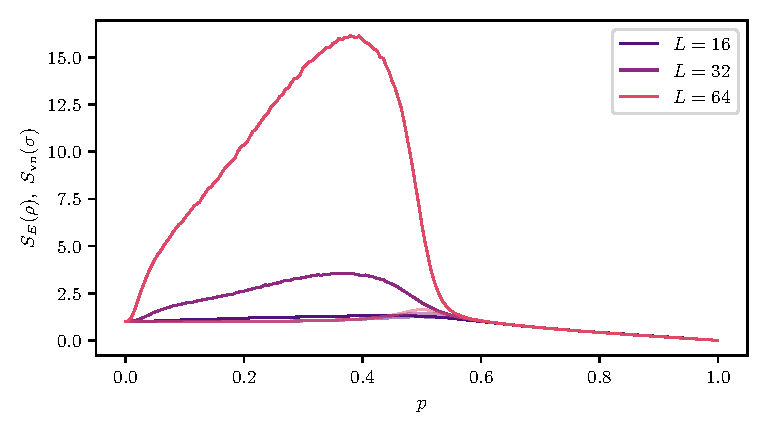
\includegraphics{naive_approach_xerrors_soloplot.pdf}
  \caption{Cross and entanglement entropy in the system with projective $X$
  errors. Measurement outcomes from a simulated experiment are projected onto a
replica in the classical simulation. If the subgroup condition is not met, we
replace the appearing infinity with $L /2$. }
  \label{fig:naive-svn-vs-se}
\end{figure}

\Cref{fig:naive-svn-vs-se} shows that the naive approach fails here already. In
the $p< p_c$ regime we often need to correct for infinities in the sample,
which get replaced, yes, but since the trivial upper bound is so far off the
actual entanglement entropy, we have this diverging behavior even for
relatively small systems, which is why only systems up to $L=64$ are shown. For
$p>p_c$ we saturate the bound again, since the $X$ noise commutes with the then
more frequently occuring $X$ measurements of the circuit, thereby restoring the
adherence to the subgroup condition.

This tells us that we need some way to cope with noise. The subgroup condition
requires us to detect the errors, since errors which are not succeeded by a
measurement (of any kind) will lead to a change in the structure of
$\mathcal{S}_\rho$, which are never detected. This undetectable change, as we
can tell from \cref{fig:naive-svn-vs-se}, happens if an error occurs on a qubit
in a state stabilized by an operator, which anticommutes with the type of
noise. For instance, if an $X$ error occurs on a qubit stabilized by $Z$. Since
$X$ measurements are more frequent for $p> 1/2$, the $X$ noise is directly
mitigated by the frequent measurements. 

What about the part where $X$ measurements aren't as frequent? We can again
estimate a probability of not detecting the altering of the stabilizers.
Imagine an error occurs in the very last layer, i.e. after all the measurements
in the circuit happened. This is the complementary probability to no errors
occuring. We thus have
\begin{align}
  P(\#\mathrm{err}>0) = 1-(1-q)^L
.\end{align}
As simple example, consider the probability of an $X$ error occuring in the
very last layer of a system with $L=32$ qubits. The probability that an error
doesn't get detected is $P\simeq\num{.275}$. Thus, about 1 in every 4 samples
would yield infinity as upper bound, which is useless. We thus make the rather
unphysical assumption that no error is allowed to happen after a certain
threshhold. As we design the circuit in a classical simulator as well, we
simply restrict the allowed errors occurring.

%\begin{itemize}
%  \item subgroup condition requires errors to be detected (and dealt with in
%    some way)
%  \item errors which are not succeeded by a measurement will lead to a change
%    in the group structure of $S_\rho$ such that $S_\sigma$ \enquote{never has
%    the chance to adapt}
%  \item maybe we should also implement some ideas from the shadow tomography
%    dings, such that errors are circumvented
%  \item Undetectable change in group structure happens if an error happens on a
%    qubit in a state stabilized by an orthogonal operator, e.g. an $X$-error if
%    the qubit is stabilized by $Z$.
%  \item The probability of any error happening in the last layer (i.e. after
%    all measurements in the circuit happenend) is $1-$ the probability of no
%    error, which is given by the binomial distribution
%    \[ P(\#\mathrm{err}>0) = 1-\binom{N}{0} (1-q)^N=1-(1-q)^N. \]
%  \item For $q=\num{0.01}$ and $N=32$ we have $P\simeq .275$
%  \item Of course, this probability says nothing about the actual simulation
%    (except for $p=0$) as it could be an error which was preceeded by an $X$
%    measurement.
%  \item That being said, you could technically compute this probability
%    analytically, by going through each layer and multiplying the probabilites
%    for \(X\) and not $ZZ$ happening to get the actual probability of failure
%   \item This is way too complicated, just to get an estimate on how many
%     simulations will end in $\infty$ for \cref{eq:kleins-ineq}. 
%\end{itemize}

%Let us now consider the information-theoretic implications of \cref{eq:cross-ent-stab}. 
Furthermore, recall that the cross entropy is a measure of the quality of an estimate of a
probability distribution \cite{coverElementsInformationTheory2006}. As we are
essentially estimating the experiment, represented by the density matrix
$\rho$, with a uniform probability distribution over the support of $\rho$, the
quality of our estimate depends only on how many events (or in this case,
states) we choose to include in our estimate. In other words, we project onto
an eigenstate $\ket{\phi}$ of $\rho$, where our estimate of the probability of
$\ket{\phi}$ is scaled by how many other states we consider with equal
probability. Alternatively, in the case where the subgroup condition is not
met, we do \emph{not} have $\ket{\phi}$ in $\mathrm{supp}\left( \sigma
\right)$. In this scenario, we project onto the $0$ vector, giving us a
divergent term in the cross entropy.
This also shows how stabilizer
states are particular in that sense. Any stabilizer density matrix we choose
for $\sigma$ will yield this result, independent of $\rho$, as long as $\rho$
is a valid density matrix. 

This means that if we were to continue with the cross entropy and the upper
bound in a pure stabilizer setting, we should think about how we could have a
finer-grained selection of values the cross entropy can take up. If we only
insert pure states, we might get lucky a couple of times, but in all
generality, we will fail to estimate the density matrix obtained in an
experiment. Thus, for the purely numerical approaches, we should abandon the
naive one in favor of reconstruction algorithms that include a broader set of
states to support $\rho$. Of course, they should, as we have been made aware by
the previous results, ensure the fulfillment of the subgroup condition as well. 

\section{Other numerical approaches}\label{sec:upperbound-numerics}

We have seen that the naive approach fails once noise comes into play.
Especially if the modelled errors are not succeeded by a measurement natively
included in the circuit. We have also noted that due to the limitations of the
stabilizer formalism, we either end up in agreement with the experiment or add
infinities to the mix. 
As we would like to stay in the stabilizer formalism, since it allows
ploynomial-time simulation of the quantum circuit in question, we need to cope
with noise in a different way, that also encompasses the tools we have at our
disposal. 

We have further found an irreconcilable limit to \cref{eq:kleins-ineq} in the
form of errors appearing in the last measurement layer. For all the further
considerations, we disallow errors after the last measurements. This is, of
course, an unphysical assumption to make, but this is, as of right now, not our
main concern, as we right now want to test the limits of \cref{eq:kleins-ineq}
on our system. This was one of them. If we relax the assumption of errors
happening everywhere, we could try other approaches and maybe get an idea of
how viable the general approach of an upper bound is to find a signature of the
entanglement transition.

The following sections introduce the methodology behind two numerical
post-processing algorithms that utilize mixed states to uphold the subgroup
condition. 
%\begin{itemize}
%  \item Naive approach fails because of errors, which cannot be detected by
%    construction
%  \item also, because so far we have only dealt with pure states.
%  \item we thus need a new classical post-processsing algorithm
%  \item first, we need to disallow errors after the last couple of
%    measurements, since these are the ones that make it into the subgroup check
%  \item this is, of course, an unphyisical assumption to take, but thats not
%    our main concern. informally speaking, we want to test the limits of
%    \cref{eq:kleins-ineq} for our system. We found this irreconcilable one in
%    the context of our model
%  \item   \item next, we have this condition of diverging cross entropy. Why not go in
%    reverse and try an algorithm, which has the stabilizers of $\sigma$ be a
%    subgroup of $\rho$.
%  \item we can do that by modifying the projections slightly
%  \item in the following sections we explore some approaches to modify the
%    projection operation to incorporate mixedness
%\end{itemize}

\subsection{Minimal Mixing}\label{sec:minimal-mixing}

The first post-processing algorithm we introduce is what one could call
\enquote{minimal mixing}. The algorithm works as follows. We start our
classical reconstruction in the same state as the initial state of the
experiment, for us it is $\dyad{GHZ+}$ in particular. Then, we project onto the
measurement outcomes where possible. In a noiseless circuit, this recovers the
standard entanglement entropy once more. Once we introduce noise this will no
longer be given. Recall the scenario shown in \cref{fig:mech-b1-lxe}. In this
case we had that the projection was successful only with probability
$1 /2$ and unsuccessful also with probability $1 /2$.

For this numerical approach, we choose to ignore the stabilizer generator with
the failed projection. That is, we replace the stabilizer by $\mathds{1}$ where
the incompatibility was detected, instead of forcing the projection. This
should, in principle uphold the subgroup condition, since we remove particular
generators from the generating set. Until it gets measured again, we have that
this stabilizer is not a generator. The technical details behind the
implementation are laid out in \cref{sec:other-dingers,alg:minimal-mixing}.

One critique that could immediately be raised at this point is the (ab)use of
mixed states in this context. Each time we come across such a discrepancy, we
throw out a generator, even though this is the most recent information we have
on the state of the system. However, we have already made some unphysical
assumptions before, and this is no exception. At this point we want to test the
performance of the upper bound in the extreme case of stabilizers and we want
to use all the tools available to us, and selectively removing stabilizer
generators from the generating set is one of them. \emph{How} we select them is
then judged by the performance of the selection in the numerical simulation.

%\begin{itemize}
%  \item We would like to compare $\rho$, which is the \enquote{experiment}
%    (i.e. a quantum simulator), with $\sigma$, which is the classical
%    simulation.
%  \item The algorithm follows a similar structure to
%    \cite{liCrossEntropyBenchmark2023}, wherein we project the measurement
%    outcomes from $\rho$ onto $\sigma$ where it is possible. The difference
%    being that we do not start with orthogonal GHZ states, but with identical
%    GHZ states. That way, there will be no incompatible measurement as long as
%    there are no errors
%  \item but what if there are errors?
%  \item consider the case that an $X$-error occurred after a $ZZ$-measurement.
%  \item Half of the time we will get an incompatible projection, which would
%    project onto the zero-vector.
%  \item In those cases, we replace the stabilizer by $\mathds{1}$, where the
%    incompatibility was detected, instead of replacing it by the measurement
%    outcome or the projection.
%  \item This ensures that the subgroup condition still holds \emph{and} that
%    subsequent measurements on the same site cannot be interfered with, i.e.
%    that this qubits stabilizer is $\mathds{1}$ until it gets measured again.
%  %\item However, we rolled a nat20 on a sleight of hand skill check: in the
%  %  cases, where we \emph{would} get $\infty$, we replace $\sigma$ (whatever
%  %  it may be at this point) by $2^{-N} \mathds{1}$
%  %\item This is also in line with the general philosophy of the density
%  %  matrix. We do not know where the error occurred, and are therefore in a
%  %  mixture of all possible quantum states
%\end{itemize}

\subsection{Maximal Mixing}\label{sec:maximal-mixing}

The next algorithm is what we could call \enquote{maximal mixing}. It is
similar to the previously introduced algorithm with the caveat that we are now
not selectively removing stabilizer generators, but removing the whole
generating set. This is the most extreme method of how one could deal with the
noise, since now once we catch it, we in principle act as if no generator of
our generating set is to be trusted. Also, as the trivial group is always a
subgroup of any group (cf. \cref{sec:grouptheory}), and as the trivial group is
generated by the empty set (cf. \cref{defn:generators}), we should most
definitely ensure the fulfillment of the subgroup condition. The technical
details behind the implementation of this algorithm is given in
\cref{sec:other-dingers,alg:maximal-mixing}.

Note that this approach should also saturate the upper bound perfectly in the
noiseless case, since we only throw out generators when we encounter a mismatch
in the projections.
%\begin{itemize}
%  \item the first approach is what we'd call \emph{maximal mixing}.
%  \item The maginot line of no errors occuring is still a factor. However, each
%    time we encounter a discrepancy for the projections, we remove \emph{all}
%    the stabilizers in $\sigma$
%  \item since the trivial group is always a subgroup of any group (group
%    axioms), we still obey the subgroup rule
%  \item the technical details are laid out in \cref{alg:maximal-mixing}
%  \item most importantly, for a system with no errors, the bound is perfectly
%    saturated, with equality everywhere
%  \item when introducing errors, we lose this feature and start to become more
%    inaccurate.
%\end{itemize}

\section{Results}\label{sec:upperbound-results}

The results to the 
\begin{itemize}
  \item The results assume knowledge of \cref{fig:err-vs-tra} and the methods
    used to obtain it.
  \item Setup is the same as in \cref{ch:lxe}, in particular, the error model
    is the same.
  \item Now we do not have orthogonal initial states!
\end{itemize}
\subsection{Minimal mixing}

\begin{itemize}
  \item \cref{fig:min_mix-svn_se-4x3} shows the upper bound, i.e. the cross
    entropy and entanglement entropy, for the minimal mixing approach
  \item minimal mixing: discarding generator, after failing to project onto
    measurement result
  \item LAST MEASUREMENTS ARE \enquote{PERFECT}, NO ERROR HAPPENS AFTER THEM.
  \item the figure is structured in a similar manner to \cref{fig:err-vs-tra},
    where in the columns we track different measurement outcomes, meaning that
    we only project onto some of them and perform measurements instead of
    projecting on the others
  \item For the \enquote{no error, track everything} case, we recover the
    identical behavior to the regular entanglement entropy
  \item For the marginalized runs, we can see that they end up in the infinite
    case rather often. This is because we measure instead of project. Thus, we
    might measure and get a random result that is orthogonal to the one we
    would have projected onto, even if there is no error present.
  \item In the case where we marginalized out $ZZ$, i.e. the \enquote{Track X}
    column, we have that for no errors, the cross entropy agrees with the
    entanglement entropy.
  \item This is because there are no $X$ measurements to track either way, so
    there is nothing that can go wrong.
  \item Once we have even the tiniest amount of $X$ measurements, everything
    goes horribly wrong
  \item Even for relatively small systems of $L=16$ and $L=32$ qubits, we
    almost always end up at the trivial upper bound of $S_E \leq 8$ and $S_E
    \leq 16$ respectively. 
  \item An interpretation in terms of quantum error correction would be that we
    did not correct an error, but rather let it happen. In a sense, this plot
    tells us that we have done a poor job correcting errors, or rather that we
    did not do so at all.
  \item In the case where we marginalized out $X$, this phenomenon is not as
    crass in its appearance. 
  \item To this end consider the plot in second column of the first row.
  \item This can be explained with the fact that we perform stabilizer
    measurements, i.e. we know where errors happened, yes, but we do not know
    the outcome of them. This is similar to the decoding threshhold
    \cite{roserDecodingProjectiveTransverse2023}, but not quite, since we do
    not know the exact state, and the procedure is different.
  \item Also, the scaling of this particular plot is exponential up to the
    critical point, where it flattens and goes to the trivial upper bound
  \item \textbf{X Errors}: In the case of $X$ errors occurring, i.e. $X$
    measurements, that we have no control over, and do not get feedback from,
    we had that the marginalized $ZZ$ / Track $X$ plot with $X$ errors.
  \item This was due to the fact that the linear cross entropy only contained
    the probabilities of success or failure, and the fact that the error type
    commuted with the tracked measurement outcomes
  \item Here, we do not have this luxury. In fact, the same things that apply
    to the case without errors applies here.
  \item We even notice that for $p=0$, there is no agreement anymore, since we
    effectively shifted the lines to the left a bit.
  \item Before, every $ZZ$ measurement was a genuine stabilizer measurement,
    since we measured generators of the stabilizer group. 
  \item This is not the case anymore, since even with $p=0$, we have sporadic
    creation and annihilation of clusters everywhere, which perturb the
    entanglement structure
  \item Thus, we do not have the same logical qubit anymore
  \item Sure, it should be corrected instantly, since we perform $ZZ$
    measurements everywhere at any time
  \item But this is not enough if errors are sufficiently frequent, which is
    the case for larger systems
  \item This is also the reason why we chose to show all these plots for
    smaller system sizes only
  \item When tracking only the outcomes of $ZZ$ measurements, we find that we
    do not have the nice exponential growth, but a superexponential growth.
  \item the occurrence of $X$ measurements, which we do not even try and
    \enquote{guess} the outcome is now larger
  \item The regime where we only have trivial upper bounds is shifted to the
    left slightly.
  \item The more interesting plot is the one where we track everything.
  \item We must have failed in our quest to bring everything under the umbrella
    of the $\mathcal{S}_\rho$ stabilizer group, since we can see a disturbing
    discrepancy between $S_E$ and the cross entropy.
  \item This discrepancy can be explained by the fact that two measurement
    layers are not enough to fully rule out undetectable errors. We can have
    clusters emerging that fit the measurement outcomes just enough so that
    they bypass our detection/error handling scheme.
  \item However, they do not bypass the subgroup check. With $X$-errors
    occurring, we, of course, correct a lot of errors, which can be seen in the
    fact that we have a tighter upper bound towards $p=0$.
  \item Closer to the critical point we find a peak, where $X$ errors are
    frequently contributing to the creation of unforseen clusters, which bypass
    the error handling scheme.
  \item We already see that we have not done enough to sanitize the input of
    the subgroup check.
  \item In the regime of $p > p_c$, we find that there is again agreement with
    the entanglement entropy, since $X$ measurements are more frequent to $ZZ$
    measurements 
    $X$ errors, such that 
  \item \textbf{ZZ Errors}:
  \item \textbf{X and ZZ Errors}: Here we have the worst of both worlds. 
\end{itemize}

\begin{figure}[p]
  \centering
  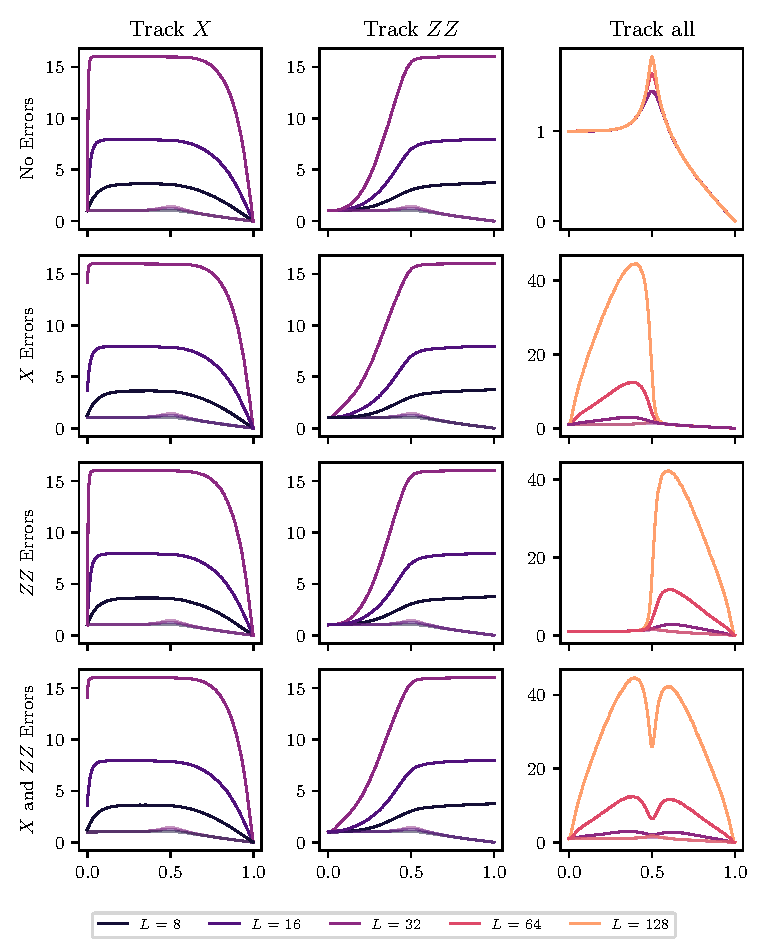
\includegraphics{minimal_mixing-4x3-svn_se.pdf}
  \caption{Cross Entropy and entanglement entropy of selected system sizes with
  periodic boundary conditions. To be able to adequately compare it to LXE the
different trackings and errors are shown in the same manner as in
\cref{fig:err-vs-tra}}
  \label{fig:min_mix-svn_se-4x3}
\end{figure}

\begin{itemize}
  \item In the simulation we trace out half the system in both cases, and then
    compute if they are subgroups of one another
  \item In case they arent, there are infinities to deal with.
  \item We deal with them by effectively replacing the algorithmically obtained
    $\sigma$ by the maximally mixed state $2^{-L /2} \mathds{1}$. That is,
    instead of adding $\infty$ (or technically, \texttt{quiet\_nan}) to the
    ensamble average, we add $L /2$.
  \item Since this is once more not how a usual physical observable behaves, we
    keep track of how often we cheat the simulation algorithm
  \item In \cref{fig:min_mix-inftyratio-4x3} we show how often we add $L /2$
    instead of $\infty$ in the data of \cref{fig:min_mix-svn_se-4x3}.
  \item This gives us an estimation on how much trickery is involved for our
    approach to not include infinities.
  \item As expected, the different marginalizations yield a high rate of
    infinities, meaning that the behavior in the corresponding subplots of \cref{fig:min_mix-svn_se-4x3} is
    largely determined by the lack of support of $\rho$ in $\sigma$.
  \item Remarkably, however, some of the group structure survives the impact in
    the case of small systems, even in the presence of errors.
  \item This can be attributed to the fact that the initial entanglement
    survivies in some cases where $p < p_c$.
  \item Note that it seems that the large values of the cross entropy in
    \cref{fig:min_mix-svn_se-4x3} in the \enquote{Track all} column really do
    seem to stem from that we replaced with another upper bound.
  \item This is yet another indicator that even in the case where we assume
    that no errors occur in the last segment of the run, we can still feel the
    pressing weight of errors
  \item Therefore, this algorithm is unfit for post-processing 
\end{itemize}

\begin{figure}[p]
  \centering
  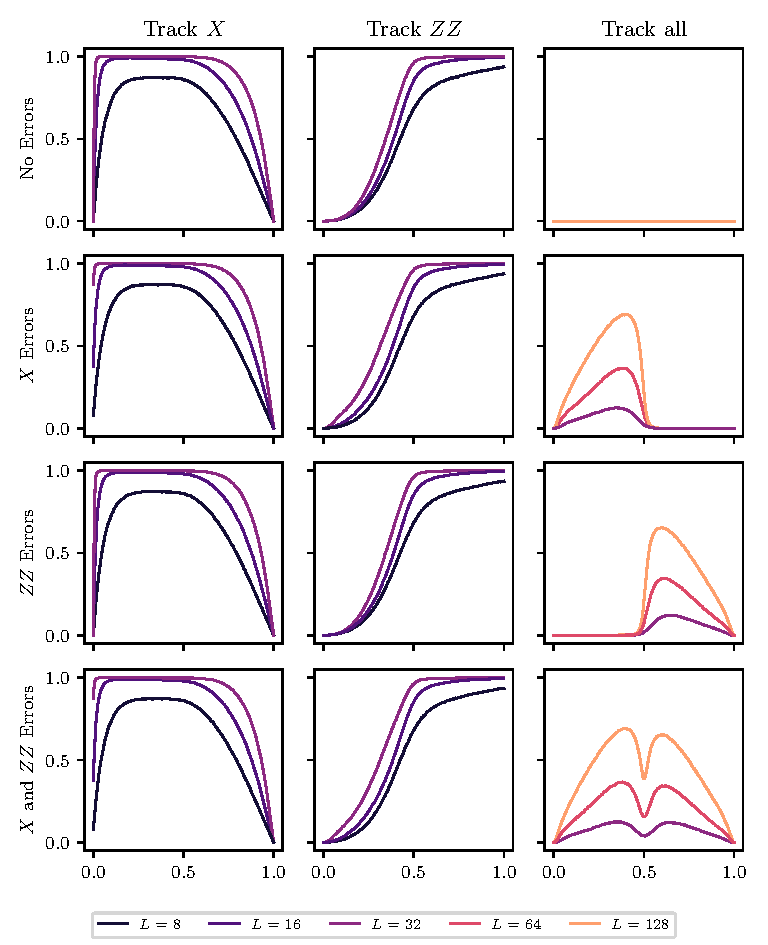
\includegraphics{minimal_mixing-4x3-inftyratio.pdf}
  \caption{Ratio of divergences in cross entropy to number of samples for
    different system sizes
  periodic boundary conditions. To be able to adequately compare it to LXE the
different trackings and errors are shown in the same manner as in
\cref{fig:err-vs-tra}}
  \label{fig:min_mix-inftyratio-4x3}
\end{figure}

\begin{itemize}
  \item As measure for how much contribution the algorithm has in the end,
    consider \cref{fig:min_mix-svn_sigma_full-4x3}, where the von Neumann
    entropy of the full density matrix of the reconstruction attempt is shown
    for all the various previous cases
  \item We can see in the \enquote{Track X} column, that there is some
    contribution from the algorithm itself, since we do not track the results
    from $ZZ$ measurements, which would interfere with projections in $X$
    towards the regime where the initial cluster dies. 
  \item For the track $ZZ$ column, we see that only when $X$ errors are
    present, 
\end{itemize}

\begin{figure}[p]
  \centering
  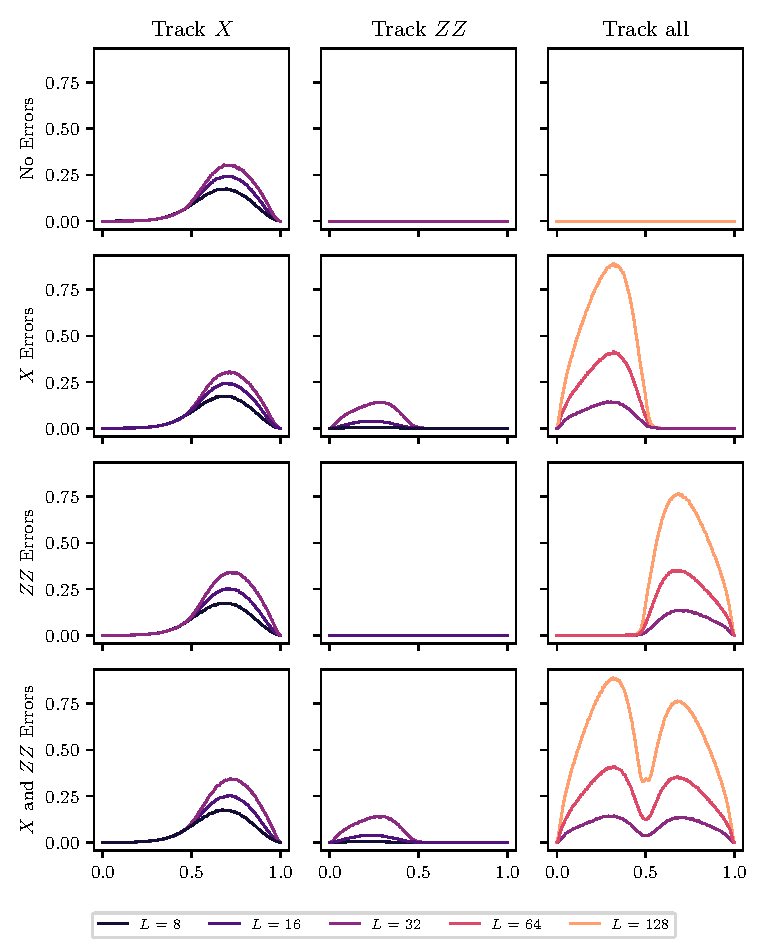
\includegraphics{minimal_mixing-4x3-svn_sigma_full.pdf}
  \caption{$S(\sigma)$ of full density matrix $\sigma$ 
  periodic boundary conditions. To be able to adequately compare it to LXE the
different trackings and errors are shown in the same manner as in
\cref{fig:err-vs-tra}}
  \label{fig:min_mix-svn_sigma_full-4x3}
\end{figure}

\subsection{Maximal mixing}
\begin{itemize}
  \item For the maximal mixing approach, we find that the first row of
    \cref{fig:max_mix-svn_se-4x3} is almost identical to the corresponding
    plots in \cref{fig:min_mix-svn_se-4x3} for the other processing
    algorithm
  \item This is due to the fact that we have not introduced errors and the
    maximal mixing procedure has no effect on this
  \item We also see that almost all the \enquote{Track $X$} or \enquote{Track
    $ZZ$} columns are similar in appearance, except for \enquote{Track $ZZ$}
    when $X$ errors are present. We will see an explanation for this in
    \cref{fig:max_mix-svn_sigma_full-4x3}, where the von Neumann entropy of the
    entire density matrices is shown.
  \item For the \enquote{Track all} columns, we have values for the cross
    entropy that are way smaller than with the previous algorithm. 
  \item When taking \cref{fig:max_mix-inftyratio-4x3} into account, we notice
    that these contributions are (almost) entirely from the post-processing
    algorithm we chose.
  \item For $X$ errors we have that the upper bound attains larger values for
    $p \approx p_c$ with a slight slant to the left
  \item the converse is true for $ZZ$ errors, where the upper bound almost
    doesn't go back to the original curve
  \item For the noisiest system with $X$ and $ZZ$ errors, we have a combination
    of the two effects
  \item Interestingly, the scaling at the critical point is linear, since the
    peaks roughly double in magnitude with doubling the system size $L$.
  \item This is in contrast to the \enquote{ideal} case, where we have
    logarithmic scaling at the critical point
  \item The peaks in the top right subplot are spaced evenly, which is as
    expected with the doubling of system size.
\end{itemize}
\begin{figure}[p]
  \centering
  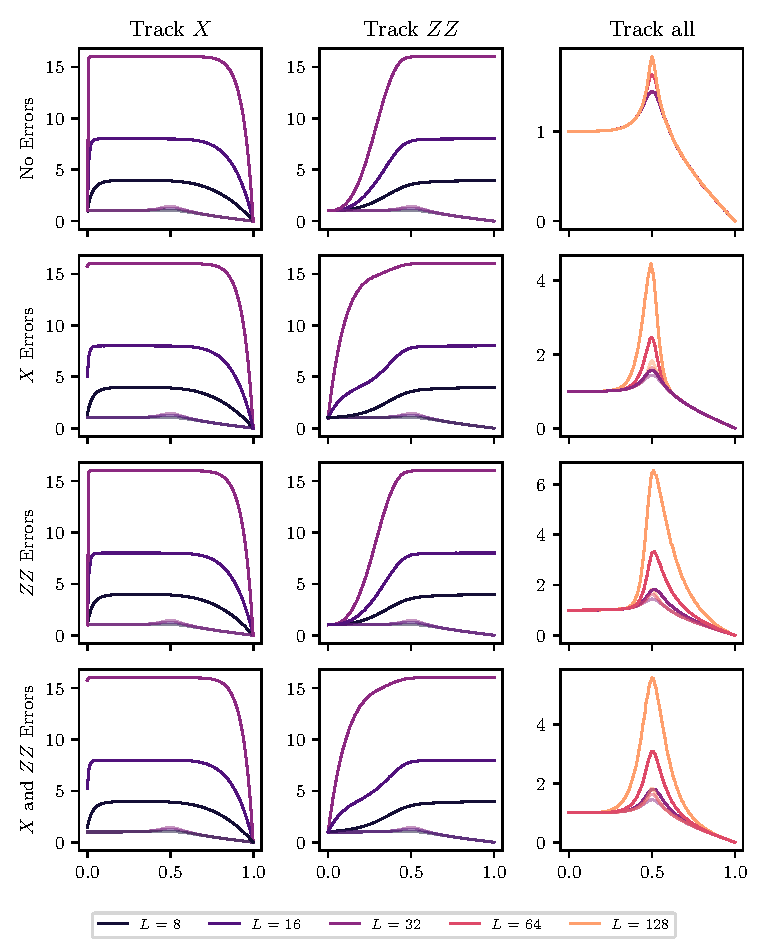
\includegraphics{extreme-rel-ent-4x3-svn_se.pdf}
  \caption{Cross Entropy and entanglement entropy of selected system sizes with
  periodic boundary conditions. To be able to adequately compare it to LXE the
different trackings and errors are shown in the same manner as in
\cref{fig:err-vs-tra}}
  \label{fig:max_mix-svn_se-4x3}
\end{figure}
\begin{itemize}
  \item For the infinity ratios, we have made progress: In the \enquote{Track
    all} column, we find that we had no infinities almost everywhere.
  \item However, there are noticeable bumps in some of the plots. They are
    miniscule, but still there. So miniscule that we can rule out the
    possibility of them substantially contributing to the behavior shown in
    \cref{fig:max_mix-svn_se-4x3}
  \item Nonetheless, this shows that even with the most extreme measure of
    trying to ensure the adherence to the subgroup condition, we still have
    some samples bypassing it.
  \item This undermines the fact that clusters emerge undetected, even within
    the last measurement layers.
  \item Consequently, we find that even when compensating with the most extreme
    measures, we do not generally comply with the subgroup condition. This
    fact rules out any purely numerical approaches to detect the phase
    transition.
\end{itemize}
\begin{figure}[p]
  \centering
  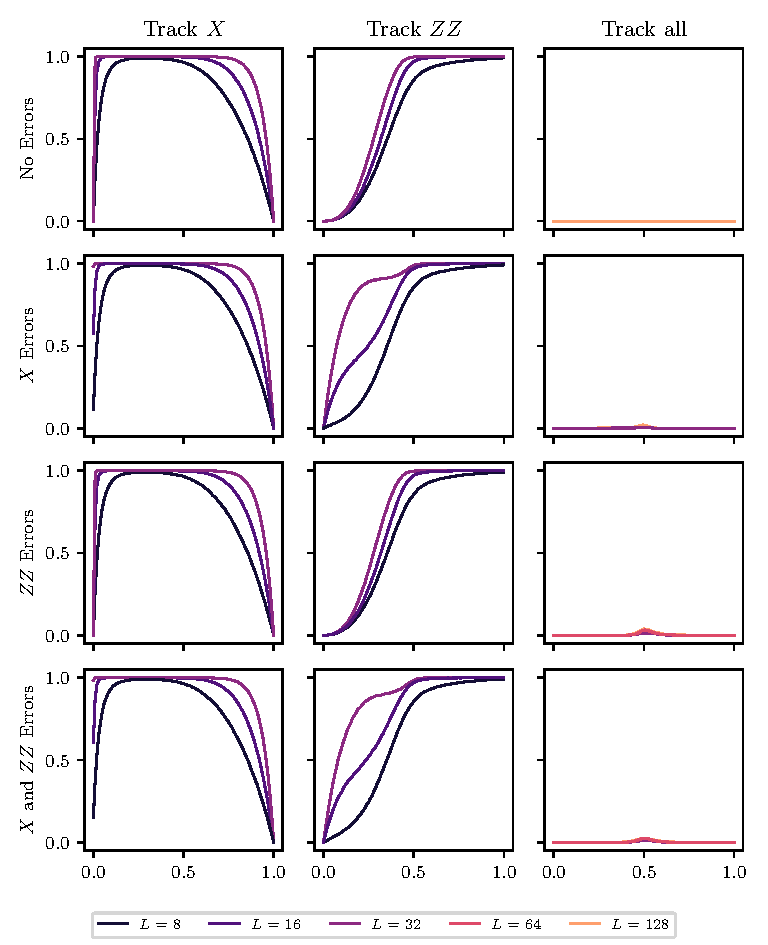
\includegraphics{extreme-rel-ent-4x3-inftyratio.pdf}
  \caption{Ratio of divergences in cross entropy to number of samples for
    different system sizes
  periodic boundary conditions. To be able to adequately compare it to LXE the
different trackings and errors are shown in the same manner as in
\cref{fig:err-vs-tra}}
  \label{fig:max_mix-inftyratio-4x3}
\end{figure}
\begin{itemize}
  \item When considering the full density matrix, we can again qualitatively
    measure how good our approach was at the very end. We see that even though
    the \enquote{mixedness} was set to the max, we never have an insanely large
    value for the von Neumann entropy, as seen in
    \cref{fig:max_mix-svn_sigma_full-4x3}.
  \item We find that for noisy systems, the algorithm did what it was designed
    to do, namely, intercept errors
  \item In the presence of $X$ errors, we almost immediately recover the whole
    group, but fail to recover the global $X$ stabilizer. This shows itself in
    the \enquote{Track all} column of \cref{fig:max_mix-svn_sigma_full-4x3},
    where it goes to $1$ for $p\to 0$.
  \item At the critical point, there is a peak for large enough systems, since
    there we have the highest impact of additional measurements of the
    competing kind.
  \item Remarkably, just as in \cref{fig:min_mix-svn_sigma_full-4x3} we have
    \enquote{$ZZ$ errors -- Track $ZZ$} be identically $0$. This follows from
    the group structure. We never maximally mix.
  \item For the \enquote{Track $X$} column, we just see the peak where the
    initial cluster dies, which was also present in
    \cref{fig:min_mix-svn_sigma_full-4x3}
\end{itemize}
\begin{figure}[p]
  \centering
  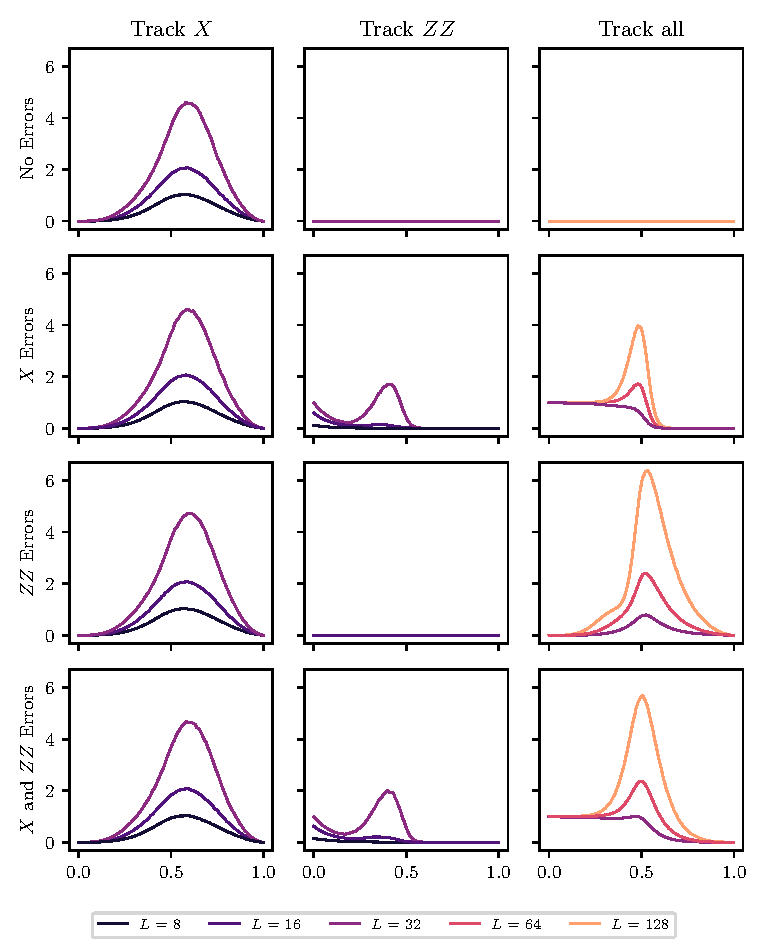
\includegraphics{extreme-rel-ent-4x3-svn_sigma_full.pdf}
  \caption{$S(\sigma)$ of full density matrix $\sigma$ 
  periodic boundary conditions. To be able to adequately compare it to LXE the
different trackings and errors are shown in the same manner as in
\cref{fig:err-vs-tra}}
  \label{fig:max_mix-svn_sigma_full-4x3}
\end{figure}

\begin{itemize}
  \item Recall that both of these simulations were based on the assumption that
    there are no errors appearing in the last measurement layer.
  \item With that we have basically thrown physics out the window
  \item However, there was still something to learn about in these simulations
    and these figures
  \item Sometimes, one needs to do some unphysical assumptions to get a better
    understanding of the physics.
  \item As a closer, we can say that the maximal mixing approach worked best,
    but not perfect, since we still can't rule out the possibility of
    divergences.
  \item For that we need to regularize
\end{itemize}
\section{Regularization}

We can see that, even though we chose our numerical algorithms in a way that
should mitigate the infinities, we still have them. Furthermore, the subgroup
check is a subtle way to incorporate once more what we try to avoid. Namely, we
want to find a density matrix, which is independent of the experimental density
matrix $\rho$. However, with the subgroup check, we implicitly introduce it
into our computation again. As we once more require knowledge of the full
density matrix, this would bring us right back to the sampling problem. In the
following we present two approaches to regularize the infinity appearing in the
cross entropy. These approaches require nothing but the numerically computed
density matrix $\sigma$. The first approach is one, which could be implemented
in a stabilizer simulator, which has the drawback of being exponentially worse
than the trivial upper bound $N$, among other things. The other is more
flexible, but lacks an efficient implementation in a stabilizer
simulation.\footnote{It is not definitive if there exists such an
implementation or not. For now, it does not exist yet.}
Note that these approaches are
designed to not need the subgroup condition to be fulfilled. As such, the
assumption of a noiseless last measurement layer could be restricted again to
include errors up to the end of measurements. 

Both of these approaches could be
the subject of further study, as the computational argument is one of
feasibility, but not possibility (i.e., it is possible, but at what
computational cost).

\subsection{Exponential Ansatz}
For the first regularization we choose an exponential Ansatz. The basic reasoning
behind this Ansatz is twofold. First, we want to ensure that the support of
$\sigma$ is large enough to contain the support of $\rho$. That is, what we
failed to achieve numerically, we attempt to achieve analytically. We want to
ensure that the classical processing step is only a function of the
measurement outcomes, $\sigma \equiv \sigma(\mathbf{m})$, and not the
experimentally obtained density matrix, which we implicitly had by checking the
subgroup condition on each run.

The second reason for this Ansatz in particular is the computability. Since we
are performing classical computations via the stabilizer formalism, we reduce
the memory requirements significantly. Storing a state of an $N$ qubit Hilbert
space is done in quadratic space complexity (cf. \cref{ch:mixed}). If we were
to write out the density matrix of, e.g., $N=100$ qubits explicitly, we would
have to deal with an exponentially large matrix. That is, if we choose $\sigma$
arbitrarily, 
we would be faced with the herculean task of diagonalizing a $2^{100} \times
2^{100}$ matrix when computing its logarithm, way beyond the scope of any reasonable computational
feasibility. By exponentiation we ensure that the logarithm \enquote{gets eaten
up} such that we are dealing with the density matrix itself with an additional
normalizing term.

As mathematical expression we may write\footnote{The factor of $\ln 2$ comes
  from the fact that we have the entropic quantities with base $2$. By a
leading factor of $1 /\ln 2$ this factor can be omitted.}
\begin{align}
  \tilde{\sigma} = \frac{\exp[\ln(2) \sigma]}{\Tr[\exp[\ln(2) \sigma]]}
.\end{align}
Substituting $\tilde{\sigma}$ back into the right hand side of
\cref{eq:kleins-ineq} we get
\begin{align}\label{eq:exp-ansatz}
  -\Tr[\rho\log\rho]\leq-\Tr[\rho\log\tilde{\sigma}] = -\Tr[\rho\sigma] +
  \log(\Tr[\exp[\ln(2)\sigma]])
.\end{align}
Note that the original $\sigma$ is still our classical reconstruction, i.e. a
density matrix in the stabilizer formalism. As $\sigma$ is therefore a product
commuting projectors, and with that a projector itself, we can once again
compute $-\Tr[\rho\sigma]$ efficiently. If $\rho=\sigma$, it recovers the
purity of $\rho$ with a negative sign, and if $\rho \perp \sigma$, then the trace is $0$. In a
sense, we here have recovered an inner product between density matrices, defined
as
\begin{align}
  \langle \rho, \sigma \rangle = \Tr[\rho\sigma]
.\end{align}
This inner product can be efficiently computed in the stabilizer formalism, as
we merely need to count projectors, and if they are orthogonal, the resulting
inner product is $0$. We remark that for density matrices, this inner product
is bounded with $\Tr[\rho\sigma] \in [0,1]$.

To efficiently compute the resulting upper bound from choosing the exponential
Ansatz, we need to resolve the logarithm in \cref{eq:exp-ansatz}. To this end
we proceed by first calculating the argument of the trace, which turns out to
yield the result of the trace as byproduct.

Since the density matrix of interest is, up to a prefactor, a projector, we
rewrite $\ln(2)\sigma$ as $c\mathbb{P}$ with some constant factor $c$.
By the matrixexponential we have
\begin{alignat*}{2}
  \exp[c\mathbb{P}] 
    = \sum_{k=0}^\infty \frac{\left(c\mathbb{P}\right)^k}{k!}
    &= \mathds{1} + \sum_{k=1}^\infty \frac{\left(c\mathbb{P}\right)^k}{k!}\\
    &= \mathds{1} + \mathbb{P}\sum_{k=1}^\infty \frac{c^k}{k!}
    &&\qquad{(\mathbb{P}^2 = \mathbb{P})}\\
    &= \mathds{1} + \mathbb{P}\left(\sum_{k=0}^\infty \frac{c^k}{k!} - 1\right)
    &&\qquad{\text{(shift index)}}\\
    &= \mathds{1} + \mathbb{P}\left(e^c -1\right) \\
    &= \mathds{1} + 2^{N-n}\sigma\left(2^{2^{n-N}}-1 \right) &&\qquad{(c =
      2^{n-N}\ln(2) \text{ and } \sigma = 2^{n-N}\mathbb{P}_s)}
.\end{alignat*}
We can then calculate the trace easily, since $\Tr[\mathds{1}] = 2^N$
and $\Tr[\sigma] = 1$. It follows that
\begin{align}
  \Tr[\exp[\ln(2)\sigma]] &= 2^N + 2^{N-n}\left(2^{2^{n-N}} -1 \right)
  \label{eq:trace-exp}
.\end{align}
Note that the parenthesis in \cref{eq:trace-exp} never vanish, but only
asymptotically reach $0$ in the thermodynamic limit. This is also the case if
one flips the sign, i.e. $\exp[-c\mathbb{P}]$, where one obtains
\begin{align}
  \Tr[\exp[\ln(2)\sigma]] &= 2^N + 2^{N-n}\left(1-2^{-2^{n-N}}\right)
.\end{align}
For both of these cases we have that the resulting upper bound is worse than
trivially assuming $N$, with diminishing fluctuations in $n$,
\begin{align}
  \log\left(\Tr[\exp[\ln(2)\sigma]]\right) &= \log(2^N +
  2^{N-n}\left(2^{2^{n-N}} -1 \right)) \geq N
.\end{align}

Since this Ansatz is worse than the trivial upper bound with variations in $n$
being small compared to the system size, we did not immediately see utility in
this approach. However, all quantities in the above calculations are
technically computable in the stabilizer simulator, and could thus be subject
of future study. 

\subsection{Rescaling probabilities}
The second regularization approach could be called the naive regularization
approach. We again want the support of $\sigma$ to span the entire Hilbert
space. With $\sigma$ being a product of projectors, it is a projector itself,
up to multiplicative factors. To complete the Hilbert space, we would need to
add the rest of the $2^{N}-2^{N-n}$ projectors needed, and rescale them in
order to put more (or less) weight on our prediction. Concretely,
we want $\sigma$ to have the form of
\begin{align}
  \tilde{\sigma} &= (1-\varepsilon)\sigma +  c\sum_{s \in
  \mathrm{ker}(\sigma)} \mathbb{P}_s \label{eq:complement-sigma}\\
&= (1-\varepsilon)\sigma +  \frac{\varepsilon}{\Tr[\sum_{s \in
\mathrm{ker}(\sigma)} \mathbb{P}_s]}\sum_{s \in
\mathrm{ker}(\sigma)} \mathbb{P}_s \label{eq:epsilon-over-trace}
,\end{align}
such that the diagonal form of $\sigma$ is
\begin{align}
  D_\sigma = \mqty(\dmat{1-\varepsilon,c,\ddots,c,c})
.\end{align}
This way, every basis vector of $H^{\otimes N}$ is included in $\sigma$ with a
weight of either $(1-\varepsilon)$ or $c$. As we want to ensure that
$\Tr[\tilde{\sigma}] =1$, $c$ is parametrized by $\varepsilon$. We now want to derive an
expression for $c(\epsilon)$, i.e. the trace in \cref{eq:epsilon-over-trace},
as well as a way to determine the constituents of the sum in
\cref{eq:complement-sigma}.

In principle, we need the sum in \cref{eq:complement-sigma} to go over all
orthogonal projections in the kernel of $\sigma$.
Since the support of $\sigma$ is fixed by the projectors onto the eigenspaces
of the tensor products of Pauli matrices contained in the generating set, we
need the orthogonal complement of each of them. Suppose we have the respective
signs of the generators $g_i$ in a bitstring $r_i$ of length $n$, i.e.
$\mathbf{r} \in \mathbb{F}^n_2$. We then write $\sigma$ as
\begin{align}
  \sigma = \frac{1}{2^N} \prod_{i=1}^n \left( \mathds{1}+(-1)^{r_i} g_i \right) 
.\end{align}
We then have a sum over all the combinations of values of $r_i$, which are
\emph{not} the original bitstring. We might write this as
\begin{align}
  \sum_{s\in\mathrm{ker}(\sigma)} \mathbb{P}_s = \sum_{\mathbf{r}' \neq \mathbf{r}} \frac{1}{2^n}\prod_{i=1}^n \left(
  \mathds{1} + (-1)^{r_i} g_i \right) 
.\end{align}
The subspaces of each of the above projectors is one-dimensional, and thus
their trace is $1$. Since there are $2^N$ total dimensions, and $2^{N-n}$ of
them are already in the support of $\sigma$, we have a total of $2^{N-n}\left(
2^n -1\right)$ additional projectors.\footnote{One can also arrive at this through
combinatorical arguments over the sign vector $\mathbf{r}$.} By rearranging and
by using the completeness relation, one can also reduce the number of
projectors needed to $\abs{\mathcal{S}_\sigma}$. However, the trace still
remains the same, since we want to rescale the missing diagonal entries
uniformly. This then yields
\begin{align}
  c = \frac{\varepsilon}{2^{N-n}\left( 2^n -1 \right) }
\end{align}
and thus
\begin{align}
  \tilde{\sigma} = (1-\varepsilon)\sigma + \frac{\varepsilon}{2^{N-n}\left( 2^n
  -1 \right) } \sum_{s\in\mathrm{ker}(\sigma)} \mathbb{P}_s
.\end{align}

Having determined a form for the auxilliary density matrix, we want to examine
it in the context of the cross entropy. It now becomes
\begin{align}
  -\Tr[\rho\log\sigma] = -\sum_n \matrixel{n}{\rho}{n} \log\lambda_n
\end{align}
with $\lambda_n =(1-\varepsilon)$ or $\lambda_n = \varepsilon
\left(2^{N-n}(2^n-1) \right)^{-1}$. While this appears to be better than the
diagonalization of a $2^{N} \times 2^{N}$ matrix, we still need to be aware
of -- or compute -- the representation of $\rho$ in the space, where $\sigma$
is diagonal.  Therefore, we do not quite dodge the task of handling an
exponentially large matrix.

%However, we can reduce this sum by realizing, that a projection onto \emph{one}
%of them halves the space which is projected onto. We can therefore build up the
%sum in the following way. First, we project onto the orthogonal space of the
%first generator, i.e.
%\begin{align}
%  \tilde{\mathbb{P}}^\perp_1 = \frac{1}{2}\left( \mathds{1} + (-1)^{1-r_1} g_1 \right) 
%.\end{align}
%Note that to ensure a uniform rescaling, we need to correct for the number of
%dimensions projected onto. In this case, we project onto a
%$2^{N-1}$-dimensional subspace.\footnote{This is a first indicator that this
%approach gets finicky.} Additionally, with said prefactor this is not a genuine
%projector anymore, since $\tilde{\mathbb{P}}^2 \neq \tilde{\mathbb{P}}$.
%
%The next one in the sum is the projector onto the space of $g_1$ multiplied by
%the orthogonal complement of $g_2$,
%\begin{align}
%  \tilde{\mathbb{P}}^\perp_2 = \frac{1}{2^{N-1}}\left(\mathds{1} + (-1)^{r_1} g_1  \right)
%  \left( \mathds{1} + (-1)^{1-r_2} g_2 \right) 
%.\end{align}
%This continues for all generators of the generating set.
%This way, we only need $\abs{\mathcal{S}_\sigma}$ projectors in the sum. 
%Since they take the form of
%\begin{align}
%  \mathbb{P}_s = \frac{1}{2}\left( \mathds{1} + s \right) 
%\end{align}
%with $s \in \mathcal{P}_N$, their trace is
%\begin{align}
%  \Tr[\mathbb{P}_s] = \frac{1}{2} 2^N = 2^{N-1}
%.\end{align}
%We argued that we only need $\abs{\mathcal{S}_\sigma}$ projectors in the sum.
%Therefore, \cref{eq:epsilon-over-trace} becomes
%\begin{align}
%  \tilde{\sigma} &= (1-\varepsilon)\sigma +
%  \frac{\varepsilon}{\abs{\mathcal{S}_\sigma}2^{N-1}}\sum_{s \in
%  \mathrm{ker}(\sigma)} \mathbb{P}_s 
%,\end{align}
%given that we choose the projectors with the above described method.


%There are $n$ generators for $\sigma$.
%
%\begin{itemize}
%  \item eigentlich sinds $2^N - 2^{N-n}$ verschiedene orthogonale projektionen,
%    die zu machen sind
%  \item gibt cleveren algorithmus wie man das reduzieren kann:
%    \begin{enumerate}
%      \item orthogonales komplement zum projektor auf den ersten
%      \item projektor auf den ersten, multipliziert mit projektor auf
%        orthogonales komplement vom zweiten
%      \item projektor auf ersten mal projektor auf zweiten mal o.k. von
%        projektor auf dritten
%      \item etc\ldots
%    \end{enumerate}
%  \item damit reduziert man erheblich, man braucht dann nur so viele wie man
%    generatoren hat, also $n$, anstatt exponentiell viele
%  \item nur doof, dass es auch daf\"ur keine gute methode gibt im stabilizer zu
%    handlen
%  \item kann sich ja der n\"achste masterand ransetzen?
%\end{itemize}

\clearpage
\section{Summary}
In this chapter we investigated the utility of Klein's inequality to detect the
entanglement transition in the projective transverse-field Ising model. This
inequality has first been employed in this manner by
\citeauthor{garrattProbingPostmeasurementEntanglement2023} in
\cite{garrattProbingPostmeasurementEntanglement2023}. 
%\section*{some relevant references}
%\begin{enumerate}
%  \item \textcolor{red}{\citetitle{aaronsonImprovedSimulationStabilizer2004}
%      fuck why didn't i read it in its entirety earlier: section 7 does the
%    job\ldots}
%  \item \citetitle{veitchResourceTheoryStabilizer2014}, entropic quantities of
%    magic states; quantifying non-stabilizerness. This paper is with gottesman
%    himself, so i thought it might be interesting to study. 
%  \item \citetitle{niekampEntropicUncertaintyRelations2012}, more or less what
%    it says. No regularization scheme or whatever. I think stabilizers are
%    mentioned tangentially, thats why i found it.
%  \item \citetitle{lashkariRelativeEntropiesConformal2014}, $\leftarrow$ me
%    grasping for straws.
%  \item \citetitle{leonePhaseTransitionStabilizer2024}, very recent, not too
%    particularily relevant to our stuff as far as i can tell.
%  \item \citetitle{wuEntanglementUpperBound2011} idfk\ldots
%  \item \citetitle{vedralEntanglementMeasuresPurification1998} one of the more
%    promising papers i've come across. probably helpful in proving the failure
%    of the na\"ive approach. However, it was published in 1998. It most likely
%    has nothing to do with stabilizers.
%  \item \citetitle{lindenQuantumEntropyCone2013}, probably some interesting
%    stuff in there, but not the thing i want.
%  \item \citetitle{buExtremalityStabilizerStates2024}, this paper is where most
%    of my confusions come from. 
%\end{enumerate}
